\def\year{2017}
\documentclass[a4paper,11pt]{report}
\usepackage{graphicx} %For images
\usepackage{times} %Font
\usepackage{booktabs}
\usepackage{multirow}
\usepackage{diagbox}
\usepackage[table,xcdraw]{xcolor}
\usepackage{amsmath,amsfonts,amsthm,amssymb}
\usepackage{cite} %For line break within citations
\usepackage[nottoc]{tocbibind} %For adding references to TOC
\usepackage{setspace} %For \onehalfspacing
\usepackage{lineno,hyperref}
\usepackage{url}
\usepackage[ruled,vlined,linesnumbered]{algorithm2e}
%\usepackage[usenames]{color}

\onehalfspacing





\newcommand\meir[1]{\textcolor{red}{meir: #1}}
\newcommand\hilla[1]{\textcolor{blue}{hilla: #1}}
\newcommand\roni[1]{\textcolor{green}{roni: #1}}


\newtheorem{definition}{Definition}
\newtheorem{theorem}{Theorem}
\newtheorem{corollary}{Corollary}
\newtheorem{lemma}{Lemma}
\newtheorem{example}{Example}



\newcommand{\argmin}{\operatornamewithlimits{argmin}}
\newcommand{\argmax}{\operatornamewithlimits{argmax}}

\newcommand{\AG}{{\tt ActionGenerator}}
\newcommand\sysrep[1]{{\tt SystemRepair(#1)}}
\newcommand{\notrep}{\overline{Repaired}}
\newcommand{\myopic}{{\tt Myopic-BRP}}
\newcommand{\astar}{A$^*$}
\newcommand{\brps}{\textit{BRP$_S$}}
\newcommand{\cost}{\textit{cost}}
\newcommand{\COMPS}{\textit{COMPS}}
\newcommand{\SD}{\textit{SD}}
\newcommand{\OBS}{\textit{OBS}}
\newcommand{\planbased}{{\tt Plan-based-BRP}}
\newcommand{\comps}{\textit{COMPS}}

\newcommand{\shortcite}{\cite}
\newcommand{\citep}{\cite}














\begin{document}
\title{\Huge{Batch Repair for Automated Troubleshooting}}
\author{Hilla Shinitzky}

\maketitle

\begin{center}
This thesis was carried out under the supervision of Dr Meir Kalech and Dr.
Roni Stern at the Department of Software and Information Systems Engineering, Ben-Gurion
University.

%This research was supported by the Israel Science Foundation (ISF) grant number 417/13.
\end{center}

\pagenumbering{roman}

\newpage

\tableofcontents \listoffigures \listoftables

\newpage

\begin{abstract}
Repairing a set of components as a \emph{batch} is often cheaper than repairing each of them separately. 
A primary reason for this is that initiating a repair action and testing the system after a repair action often incurs non-negligible overhead. 
However, most work so far on troubleshooting algorithms neglected to consider 
this option of performing a \emph{batch repair} action. 
In this work we close this gap, and address the problem of choosing which batch of components to repair so as to minimize the overall repair costs. We call this problem the \emph{Batch Repair Problem} (BRP) and formalize it. Then, we propose several heuristic algorithms for solving it, and a potentially optimal algorithm based on formulating this problem as a Markov Decision Problem (MDP). 
Experimentally, we show the benefit of all algorithms over repairing components one at a time, and the benefit of the algorithms we suggested for choosing these set of components to repair.
\end{abstract}

\pagenumbering{arabic}

\chapter{Introduction}
\label{sec:introduction}
% Troubleshooting, but have repair overhead
Troubleshooting algorithms, in general, plan a sequence of actions that are intended to fix an abnormally behaving system. Fixing a system includes performing \emph{repair action} in order to repair faulty components. Such repair actions incur a cost. These costs can be partitioned into two types of repair cost. The first, referred to as the {\em component repair cost}, is the cost of repairing a component. The second, referred to as the {\em repair overhead}, is the cost of preparing the system to perform repair actions (e.g., halting the system) as well as the cost of testing the system after performing the repair action.

% Thus, batch repair makes sense. Introducing BRP
This paper considers the case where the repair overhead is not negligible and is potentially more expensive than a component repair cost (of a single component). 
Therefore, it may be more efficient to repair a \emph{batch} of components in a single repair action. 
In fact, repairing a single component at a time can be wasteful even if that component is the most likely to be faulty. Consider cases where all the found diagnoses consist of multiple faulty components. Having only diagnoses that represent multiple faults suggests that repairing a single component will not fix the problem. Thus, it may be more effective to choose to repair the components in the single most likely diagnosis. Moreover, it may even be worthwhile to repair, in a single repair action, a set of components that ``covers'' more than a single diagnosis. This may reduce the number of repair actions until the system is fixed, thus saving repair overhead costs. 

%The downside in this approach is that healthy components may be repaired, increasing the overall repair costs.
%\meir{I motivated it by a real world example which I moved from the next para to here} 
%For example, if a diagnosis engine infers that multiple faulty components need to be repaired to fix the system, then it would be wasteful to repair these components one at a time since each repair action incurring its repair overhead. \roni{The "For example," part does not add any information. It is not an example, you are just saying the same thing again. I suggest you simply remove it.}
% Previous work did not try to batch-repair. We need a cost-effective solution that does.

Nonetheless, most previous work assume that components are repaired one at a time \cite{heckerman1995decision,friedrich1992choosing,Nyberg12,Torta14}. Considering batch repair actions raises 
the problem of choosing which batch of components to repair. 
We call this problem the Batch Repair Problem (BRP). BRP is an optimization problem, where the task is to minimize the {\em total repair costs}, which is the sum of component repair costs and costs due to repair overheads incurred by repair actions performed until the system is fixed. \footnote{% Terminology : fix and repair
Note that in this paper we use the term  ``fix'' when referring to the entire system and term ``repair'' for a single or a set of components.  Thus, 
to {\em fix} the system one needs to {\em repair} components, and a system is only fixed if it returned to its nominal behavior.}



%This approach can be wasteful.\roni{Explain why it is wasteful. If you add earlier in the paper an example, you can point to it}
%for BRP. For example, if a diagnosis engine infers that multiple faulty components need to be repaired to fix the system, then it would be wasteful to repair these components one at a time since each repair action incurring its repair overhead. Instead, an efficient BRP algorithm would repair all the faulty components in a single repair action. More generally, %We expect an intelligent BRP algorithm to consider  repair overheads and the component repair costs when deciding which components to repair. 
% Why is BRP hard.


 %the component repair costs can be high, as more healthy components may be repaired.


\begin{figure}{}%{4cm}
\begin{center}
  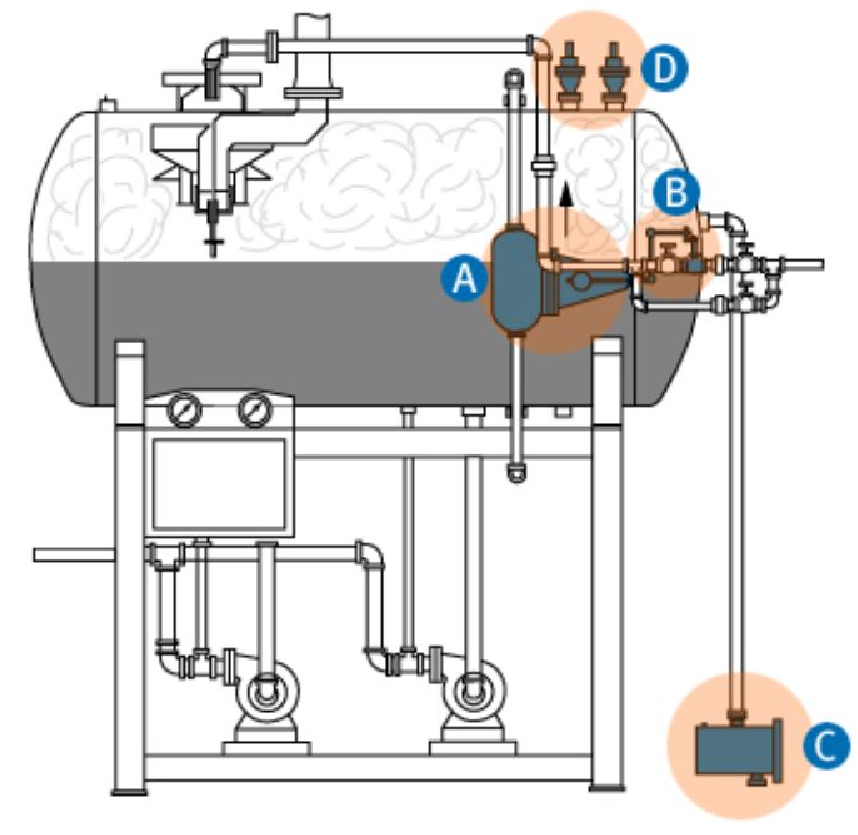
\includegraphics[width=0.5\columnwidth]{system_example.pdf}
  \caption{An example where repairing components one at a time is wasteful.}
  \label{fig:simple-example}
\end{center}
\end{figure}

To demonstrate the BRP problem, consider the system depicted in Figure~\ref{fig:simple-example}, which is a boiler tank system scheme made by Warren Controls, Inc. When demand for water reduces the liquid level in the tank, the float cage ($A$) opens the lever valves ($B$) to supply intake water to the tank and closes it when the water reaches the desired level. Component $C$ is an overflow trap that collects and relieves condensate overflow. Component $D$ includes two vacuum breakers which are opened to relieve the tank with outside air to prevent vacuum pressures in the tank.

Assume some water was extracted from the tank, and so additional water is required, but we observe that the water level does not increase. There are two possible diagnoses: either the float cage $A$ is faulty or the lever valve $B$ is faulty. Assume that the probabilities of $A$ and $B$ to be faulty are given by the manufacturer and are 0.06 and 0.04, respectively. Since only these diagnoses can explain the problem, the normalized probability of $A$ to cause the problem is 0.6 and that of $B$ is 0.4. There are three possible repair actions: to repair $A$, to repair $B$, and to repair $A$ and $B$. Assume the repair cost of each component is 5\$ but the repair overhead is 50\$, due to the cost of opening the tank and boiling the water. If $A$ is repaired, there is a 0.4 chance that the system would not be fixed and another repair action would be needed (repairing $B$). Thus, the expected total repair cost of repairing $A$ first is $0.4\cdot(5+50)+5+50=77$. Similarly, the total repair cost for repairing $B$ first is $0.6\cdot(5+50)+5+50=88$. The best option is thus to repair $A$ and $B$ together in a single repair action, incurring a total repair cost of $5+5+50=60$.


%\roni{I think that we do more than modeling it as a combinatorial optimization problem. You also model it as an MDP. The paragraph below needs to be fixed to address this.} - hilla: done
In this work we model BRP as a combinatorial optimization problem, searching in the combinatorial space of possible repair actions for the best repair action. There are two challenges in implementing this approach: (1) how to measure the quality of a repair action, and (2) how to efficiently search for the repair action that maximizes this measure. There are many efficient heuristic search algorithms in the literature, and thus we propose intelligent heuristics for estimating the merit of a repair action. In addition we cope with the second challenge by proposing greedy and optimal heuristic search and planning algorithms.
In addition, we model BRP as Markov Decision Process (MDP), where the idea is to look further into the future and by that attempt on assessing which repair action could be resulted with the lowest repair costs. 

We evaluate the effectiveness of the heuristics for estimating the merit of a repair action as well as the search algorithms experimentally on two different benchmarks. The first is a standard Boolean circuit systems, which is a commonly used benchmark in the troubleshooting line of work. The second benchmark we have experimented on contains randomly generated observation from the medical physiotherapy field.
A clear observation from the results is that indeed considering batch repair actions can save repair cost significantly and that intelligent heuristics are crucial in saving repair costs. 


\chapter{Related Work}
\label{sec:relatedWork}	
BRP is a troubleshooting problem, where the goal is to perform repair actions in order to fix an abnormally behaving system. Algorithms for automated troubleshooting were proposed in previous works. Most previous work assumed that components are repaired one at a time ~\citep{heckerman1995decision,friedrich1992choosing,Nyberg12,Torta14}. This approach can be wasteful for BRP. For example, if a diagnosis engine infers that multiple faulty components need to be repaired to fix the system, then it would be wasteful to repair these components one at a time since each repair action incurring its repair overhead. Instead, an efficient BRP algorithm would repair all the faulty components in a single repair action. 
In troubleshooting, there are two main areas. The first is the Diagnosis, which focuses on the part in the troubleshooting process that searches the possibilities of explanations to what could have cause the system's malfunction. The second is the Planner, which focuses on planning the actions that follows the diagnosis phase, such as reducing the number of diagnoses, deciding what will be the next repair action etc. This chapter will present related work from various areas and lines of works in troubleshooting. The first part of this chapter will discuss about related troubleshooting processes and algorithms. The second part will present diagnosis approaches, while focusing on the field of Model-Based Diagnosis. Finally, the last part will present related work from the planning filed and will elaborate about different planner algorithms and approaches. 

\section{Diagnosis Approaches}

%\subsection{General Diagnosis Approaches}
There are diverse diagnosis approaches such as data-driven, case-based reasoning, and model-based diagnosis.
Data-driven approaches are model-free statistical methods, which attempt to learn relations between the symptoms and the faults ~\cite{murray2005machine}. These methods face the challenge of a dependency of the existence of quality information that can be extracted from the data. One disadvantage of most works in this approach is that they learn only a single fault rather than multiple faults. In addition, inductive learning methods do not guarantee sound diagnoses nor completeness.
Another approach is case-based reasoning. Experts often find it easier to relate stories about past cases rather than to formulate rules. Case-based reasoning approaches keep a repository of cases and their appropriate diagnosis. When a new case appears the case-based reasoning system tries to find the most similar case from the repository in order to adapt the relevant diagnosis ~\cite{aamodt1994case}. The main assumption is that similar problems have similar solutions. Similar to data-driven approaches, this approach also does not guarantee sound diagnoses nor completeness. Thus, one could not be certain that the resulting diagnosis is indeed the faulty component.
In this work we focus on model-based diagnosis approach ~\cite{reiter1987theory}.

%\subsection{Model-Based Diagnosis}
In MBD we must have a precise model of the system. MBD relies on a model of the diagnosed system to compute the expected behavior of the system. When the expected and observed behavior differs, the model is used to infer possible failing components ~\cite{reiter1987theory}.
The Model Based Diagnosis problem with weak fault model has been widely researched and a wide range of papers propose different algorithms to solve it ~\cite{reiter1987theory,de1987diagnosing,williams2007conflict,feldman2010approximate,siddiqi2007hierarchical}.%Till today it is considered a challenge as reflected by the “synthetic track” in the annual DXC diagnosis competition [20].
Many of the existing diagnosis techniques propose to apply a combination of deterministic reasoning and search algorithms. One classic approach involves a two stage process. First, it identifies conflict sets, each of which includes at least one fault. Then, it applies a hitting set algorithm to compute sets of multiple faults that explain the observation~\cite{de1987diagnosing,williams2007conflict}. These methods guarantee sound diagnoses, and some of them are even complete. However, they tend to fail for large systems due to infeasible runtime or space requirements.
Compilation-based methods have also been proposed in the MBD context. Torasso and Torta apply binary decision diagrams (BDD) to compile the model ~\cite{torasso2006model}. Darwiche ~\cite{darwiche2001decomposable} compiles a system description into Decomposable Negation Normal Form (DNNF) where a minimal cardinality diagnosis can be found in time that is polynomial in the size of the DNNF. This compilation approach is attractive because inference of diagnoses can typically be done in time that is linear in the size of the compiled representation; however, there is no guarantee that the size of the compiled representation will not be exponential in the number of system components. Other work proposes to compile MBD to the SAT problem ~\cite{metodi2012compiling}, and then use state-of-the-art SAT or MAX-SAT solvers to find the possible diagnoses. 
In this work, in order to find the possible faulty components, we will use the MBD approach in the implementation of the diagnosis engine.  

\section{Troubleshooting Planner}
There are two lines of work that studies planning algorithms in the context of troubleshooting. The first is probing and testing which are the two known methods for reducing the number of diagnoses after they are found. In the second line of work, there is a use of planning in order to decide which possible repair actions can be taken next. BRP algorithms are a part of the second line of work. 

\subsection{Probing and Testing}
Some methods try to deal with reducing the number of diagnoses after they are found. There are two known methods to discriminate diagnoses, either by testing or probing ~\cite{de1987diagnosing} . In the testing method the diagnosis process is run through additional input vectors. Under the assumption that faulty components in the system remain permanently faulty along different input vectors, diagnoses that are inconsistent with multiple observations can be pruned. The probing task is similar, but instead of running the diagnosis on a new input vector, the probes are requests on the observation of the output of internal components. Probes can prune diagnoses that are not consistent with the new internal observation. Both methods can be run iteratively until focusing on a single diagnosis.
Zamir, Stren and Kalech~\cite{zamir2014using} proposed a combination of AI techniques to improve software testing. In this domain, the diagnoses represents a set of possible explanations to a failed test, and a planning algorithm is used to suggest further tests to identify the correct diagnosis. They describing an iterative course of action which prunes incorrect diagnoses in each iteration while using an MBD algorithm. This iterative process, which they call Test, Diagnose and Plan (TDP), continues until the correct diagnosis is returned. Several test planning algorithms are proposed to minimize the number of TDP iteration, and consequently the number of tests required until the correct diagnosis is found. 
Torta et al.~\cite{Torta14} proposed using model abstractions for troubleshooting and point out the role of abstractions in an iterative abduction process. Similar to Model-Based Diagnosis and troubleshooting, at each iteration of the abduction process the proposed algorithm in their work chooses to perform further observations or actions taking into account their costs and the likelihood candidate hypotheses. %BRP algorithms also uses the costs and likelihoods, thus these values have a major influence on the decision of which components to repair. 
The planning role in the troubleshooting processes described above is to reduce the number of diagnoses by finding and pruning incorrect ones. In the BRP the goal of the planning algorithms in each iteration of the troubleshooting process is to find the right component to repair so the system will be fixed as soon as possible, meaning eventually fixing all the correct diagnosis' components. 


\subsection{DTT Planner}

%\roni{you already mention this planner above. The structure of the related work section needs work. Try to make it more coherent. Start with the diagnosis stuff, then the troubleshooting.} hilla-done

Heckerman et al.~\cite{heckerman1995decision} proposed the decision-theoretic troubleshooting (DTT) algorithm that uses a decision theoretic approach for deciding which components to observe in order to identify the faulty component. Later work also applied a decision theoretic approach that integrated planning and diagnosis to a real world troubleshooting application~\cite{Nyberg12,warnquist2009planning}. 
The diagnostic procedure developed by Heckerman et al.~\cite{heckerman1995decision} not only seeks to identify the most likely causes of a malfunction, but also generates a plan of action for repair. This plan consists of repairing or replacing individual components of a composite device or system, as well as making observations or tests. This is essentially the troubleshooting process. An optimal troubleshooting plan, as described in their work, is a sequence of observations and repairs that minimizes expected costs. The classic way to compute the expected cost of a plan is to use a decision tree. The decision tree contains: decision nodes that represents of whether or not to observe variable o, chance nodes of each o which represents an observation that provides some evidence about the status of the components and its branches represent the possible outcomes of the variable, and decision nodes that represents the decision of whether or not to fix the component c. The values at the end of the tree are cumulative costs of observation and repair along the path from the root. The expected cost of a troubleshooting plan is computed by rolling back a decision tree from right to left – a particular form of dynamic programming. After all the computations has been done, there will be a chosen action for each decision node and ultimately will represent the optimal plan. 
The possible decisions that can be made, after assembling the optimal plan derived from a decision tree, can only integrate repair action that contains only one component. In BRP, the idea is to consider repairing more than one component in each repair action. The decision tree grows exponentially as the problem grows. This applies for cases in which the upper bound of the amount of possible repair actions is the number of components. Imagine how the tree will look like in cases, such as BRP, where the amount of possible repair actions that is exponential with the number of components. In other words, using decision tree to solve BRP in most cases is not feasible. 
Pernest{\aa}l et al. ~\cite{Nyberg12} work was motivated by the task of repairing an automotive vehicle at lowest possible expected cost, and proposed a decision theoretic troubleshooting system that is developed to handle external interventions. Warnquist et al.~\cite{warnquist2009planning} studied the problem of incremental fault diagnosis and repair of mechatronic systems where the task is to choose actions such that the expected cost of repair is minimal. This is done by interleaving acting with the generation of partial conditional plans used to decide the next action.

\subsection{Breakdown Costs}
Some of the previous works in this line of work considered also the costs. Friedrich and Nedjl~\cite{friedrich1992choosing} discussed the relation between diagnoses and repair, in an effort to minimize the breakdown costs. Breakdown costs roughly correspond to a penalty incurred for every faulty output in the system, for every time step until the system is fixed. In BRP, the goal is to minimize costs until the system if fixed, and there is no partial credit for repairing only some of the system outputs.

%\section{}

None of these works considered the possibility of repairing a set of components together, allowing only repair actions that repair a single component at a time.
%\roni{Remove the next two paragraphs. Your thesis summarizes all our work. You don't need to discuss how it relates to some preliminary workshop paper that we did}
%Recent work of Stern and Kalech~\cite{stern2015repair} proposed two high-level approaches to solve BRP: as a planning under uncertainty problem, or as a combinatorial optimization problem. When modeling BRP as a planning under uncertainty problem the task is to find a repair policy, mapping a state of the system to the repair action that minimizes the expected total repair costs. This approach, while attractive theoretically, quickly becomes not feasible in non-trivial scenarios.
This work do not consider applying further diagnostic actions such as probing and testing, which are considered by previous troubleshooting algorithms. Thus, this work could be integrated in previous troubleshooting frameworks in order to consider both batch repair actions and diagnostic actions. This is left to future work.



\chapter{Problem Definition}

%\roni{There is a bit of a mish-mash. Now you define MBD,then stop talking about it for a while and define BRP, then stop talking about BRP while and talk about diagnoses, and then talk about BRP.I recommend: say in the beginning that BRP is related to MBD. Then define MBD, diagnoses, MBDE and all that is not BRP. Only then define BRP properly.} 
%\hilla{done}

In this section we define the batch repair problem and provide relevant background. 
I is important to lay the base for defining BRP, by presenting the related definitions of MBD. 

\section{MBD}
Following standard model-based diagnosis (MBD) terminology, we denote by $\COMPS$ and $\OBS$ the components in the system and the observed system behavior, respectively. $\SD$ describes the behavior of the diagnosed system, and in particular the behavior of each component. The term {\em behavior mode} of a component refers to a state of the component that affects its behavior. $\SD$ describes for every component one or more behavior modes. For every component, at least one of the behavior modes must represent the nominal behavior of the component. The normal mode is often described by the clause $h(C_i) \rightarrow \varphi_{C_i}$, where $C_i\in \COMPS$. $h(C_i)$ is a predicate stating that $C_i$ is healthy, and $\varphi_{C_i}$ describes the nominal behavior of $C_i$. For instance, the nominal behavior of the lever valve (component $B$ in Figure \ref{fig:simple-example}) is to be opened once the float cage opens it, while an abnormal behavior can be stuck open or close.

A mode assignment $\omega$ is an assignment of {\em behavior modes} to components. Let $\omega^{(+)}$ be the set of components assigned a nominal (i.e., normal) behavior mode and $\omega^{(-)}$ be the set of components assigned one of the other modes.

\begin{definition}[Diagnosis]
A mode assignment $\omega$ is called a diagnosis if $\omega \wedge \OBS \wedge \SD$ is satisfiable.
\end{definition}

\section{MBDE}
A model-based diagnosis engine (MBDE) accepts as input $\SD$, $\OBS$, and $\COMPS$ and outputs a set of diagnoses $\Omega$. A diagnosis $\omega$ is {\em correct} if by repairing the set of components in $\omega^{(-)}$ the system is fixed. Although a diagnosis is consistent with $\SD$ and $\OBS$, it may be incorrect. 

%\roni{1. You use the term ``incorrect'' for a diagnosis, but only explain what is a ``correct'' diagnoses the sentence after. Reverse the order. 2. I don't think your definition of ``correct'' is good, as it means that the diagnosis that contain all the components in the system is also ``correct''. I think in a ``correct'' diagnosis it also must be that no subset of it will result in a fixed system. } hilla- I can add a definition of subset minimal diagnosis - done

Notice that according to the definition above, a diagnosis which contains all the system's components, $\omega = \COMPS$, is also considered to be {\em correct}. 
Some MBDE returns only the Subset-Minimal diagnoses. A diagnosis $\omega$ is defined as a Subset-Minimal if there is no subset of $\omega$ which by repairing only this set of components will resulted with a fixed system. In our work, we use a MBDE that generates only Subset-Minimal diagnoses.

Some diagnosis algorithms return, in addition to $\Omega$, a measure of the likelihood that each diagnosis is {\em correct}~\cite{williams2007conflict,abreu2011simultaneousDebugging,Stern15shely}. Let $p: \Omega \rightarrow [0,1]$ denote this likelihood measure. We assume that $p(\omega)$ is normalized so that $\sum_{\omega\in\Omega} p(\omega)=1$ and use it to approximate the probability that $\omega$ is correct.

A common way to estimate the likelihood of diagnoses, assumes that each component has a prior on the likelihood that it would fail, denoted $p(c)$, and components fail independently ~\cite{Stern17shelly}. 
Under these assumptions, the likelihood of a diagnosis can be computed as
\begin{equation}
\displaystyle p(\omega)=\frac{\prod_{c\in\omega^{-}} p(c)}{\sum_{\omega'\in\Omega}{\prod_{c\in\omega'^{-}} p(c)}}
\label{eq:likelihoods}
\end{equation}
where the denominator is a normalizing factor. 
In our experiments we computed diagnoses likelihoods computed according to Equation~\ref{eq:likelihoods}, 
but other methods for computing likelihood of diagnoses also exist~\cite{mengshoel2010probabilistic} and the algorithms we propose are agnostic to how these probabilities are found. 


\section{BRP}

A {\em batch repair problem} (BRP) arises when the assumption that all components are normal is not consistent with the system description and observations. Formally,
\[ \SD \wedge \OBS \wedge \bigwedge_{C\in \COMPS} h(C) ~~~ \text{is not consistent} \]

In the example shown in Figure \ref{fig:simple-example}, assuming that all components are healthy under the observation that the water level is decreased is not consistent. Then a possible diagnosis is that components $A$, $C$ and $D$ are healthy, while $B$ is in an abnormal mode. For instance, the lever valve ($B$) is stuck close. Another possible diagnosis is that $B$, $C$ and $D$ are healthy, while $A$ is in an abnormal mode. In order to get the system to function correctly, at least one component must be repaired.

\begin{definition}[Repair Action]
A repair action can be applied to any subset of components and results in these components becoming normal. Applying a repair action to a set of components $\gamma$ is denoted by Repair($\gamma$).
\label{def:repairAction}
\end{definition}
\noindent ~\ref{def:repairAction} assumes that repair actions always succeed, i.e., a component is normal after it is repaired. 

After a repair action, the system is tested to check if it has been fixed.
We assume that the system inputs in this test are the same as in the original observations ( $\OBS$ ). The observed system outputs are then compared to the expected system outputs of a healthy system. Thus, the result of a repair action is either that the system is fixed, or a new observation that may help choosing future repair actions.

Repairing a set of components incurs a cost, composed of a repair overhead and component repair costs. The repair overhead is denoted by $\cost_{repair}$, and the component repair cost of a component $c\in \COMPS$ is denoted by $\cost_{c}$.

\begin{definition}[Repair Costs]
Given a set of components $\gamma\subseteq \COMPS$, applying a repair action Repair($\gamma$) incurs a cost:
\[ \cost(Repair(\gamma)) = \cost_{repair} + \sum_{c\in \gamma} \cost_{c} \]
\end{definition}
We assume that all repair costs are positive and non-zero, i.e., $\cost_{repair}>0$ and $\cost_{c}>0$ for every component $c \in \COMPS$. As defined earlier, the task in BRP is to fix a system with minimum total repair cost.

As shown in Figure~\ref{fig:simple-example}, an efficient BRP solver should consider the possibility of repairing a set of components in a single repair action. Thus, the potential number of repair actions is %exponential in the number of components, in particular the power set of the components
$2^{|\COMPS|}$. Therefore, from a complexity point of view BRP is an extremely hard problem.


\subsection{System Repair Likelihood}\label{sec:Repair_Likelihood}
If the MBDE returns a single diagnosis $\omega$ that is guaranteed to be correct, then the optimal solution to BRP would be to perform a single repair action: Repair($\omega^{-})$. 
This, however, is rarely the case, and more often possibly a very large set of diagnoses is returned by diagnosis algorithms. This introduces uncertainty as to whether a repair action would actually fix the system. We define this uncertainty as follows:

\begin{definition}[System Repair Likelihood]
The System Repair Likelihood of a set of components $\gamma\subseteq \COMPS$, denoted \sysrep{$\gamma$}, is the probability that Repair($\gamma$) would fix the system.
\end{definition}

Consider the relation between $p(\omega)$ and \sysrep{$\omega$}. If $\omega$ is correct, then repairing all components that are faulty, meaning $\omega^{(-)}$, would fix the system. Therefore, the likelihood of repairing $\omega^{(-)}$ causing the system to be fixed is at least $p(\omega)$, i.e.,
\[ \sysrep{\omega^{(-)}}\geq p(\omega)  \]
Moreover, if $\omega$ is correct then repairing any superset of $\omega^{(-)}$ would also fix the system. Thus, $\sysrep{\omega^{(-)}}$ may be larger than $p(\omega)$.
On the other hand, repairing any set of components that is not a superset of $\omega^{(-)}$, as there would still be faulty components in the system.
Therefore, a repair action Repair($\COMPS '$) would fix the system if and only if $\omega^{*{(-)}}\subseteq \COMPS '$, where $\omega^*$ is the correct diagnosis.
While we do not know $\omega^*$, we can compute \sysrep{$\gamma$} from $\Omega$ and $p(\cdot)$:
\[ \sysrep{\gamma} = \sum_{\omega\in \Omega \wedge \omega\subseteq \gamma} p(\omega) \]
\sloppy{For example, in the boiler tank depicted in Figure~\ref{fig:simple-example}, there are two diagnoses, $\{A\}$ and $\{B\}$, such that $p(\{A\})=0.6$ and $p(\{B\})=0.4$. Thus, $\sysrep{\{A\}}$=0.6, $\sysrep{\{B\}}$=0.4, and $\sysrep{\{A,B\}}$=$p(\{A\})$+$p(\{B\})$=1.}

\subsection{System State During Repair}
\label{sec:sysStateDuring}
Fixing a system involves potentially many repair actions. We use the term {\bf repair process} to refer to the process of applying these sets of repair actions until the system is fixed.
During the repair process, two sets are maintained. 
{\bf Repaired:} the set of components already repaired, 
{\bf Observed:} the set of observations, including $OBS$ as well as all the additional observations obtained after performing a repair action. 
We use the term {\bf system state} to refer to the values of Repaired and Observed at a given point in time during the repair process. For a given system state, we denote by $\overline{Repaired}$ as the set of components that were not repaired yet, i.e., $\overline{Repaired} = COMPS \setminus Repaired$. Following standard mathematical notation, we denote by $2^{\overline{Repaired}}$ as the set consisting of $\overline{Repaired}$ and any of its subsets. As there is no need to repair a component twice to fix the system, only repair actions that repair a set of components that is a member of $2^{\overline{Repaired}}$ should be considered.

\chapter{BRP as a Combinatorial Search}
As mentioned in the introduction, one of our proposed approaches for solving BRP formulates BRP as a combinatorial search problem. In this section we propose several algorithms for solving BRP as a combinatorial search problem.
%\roni{No. We also checked other options (MDP). You can write here that in this section we propose several algorithms for solving BRP that cast BRP as a combinatorial search problem. }
The search space is the space of possible repair actions, i.e., every subset of the set of components there were not repaired yet. We aim to search for the \emph{best} batch repair action. To this end, we need a search algorithm to search in the space of all possible batch repair actions, and we need a utility function to evaluate the merit of a batch repair action, so that the best repair action is the one that maximize this utility function. Thus, The effectiveness of this search-based approach for BRP depends on the search algorithm used and how the utility function is defined. 
%In the following subsection we propose several utility functions. 


%\roni{This is hard to follow. Think about the reader: what is $u(\cdot)$? you explain this later, but at this stage the reader is puzzled. My recommendation: explain our approach in a high level first:  we aim to search for the \emph{best} batch repair action. To this end, we need a search algorithm to search in the space of all possible batch repair actions,  and we need a utility function to evaluate the merit of a batch repair action, so that the best repair action is the one that maximize this utility function.}

% Myopic is still hard
%Implementing this search-based approach for BRP requires defining $u(\cdot)$ and defining a search algorithm used to search for the best repair action.

%There are many existing heuristic search algorithm for searching large combinatorial search spaces~\cite{russell2010artificialIntelligence,edelkamp2011heuristic}. Next, we propose several utility functions. 
%Thus, in this work we propose and evaluate a set of possible utility functions.  \roni{Really? I remember you also evaluate many search algorithms. I recommend: ``Next''} Note that for some of the utility functions described next it is possible to find the best repair action without searching the entire search space of possible actions, while others are more computationally intensive.

\section{Utility Functions} 
As explained above, the search problem comes down to finding the repair action that maximizes a utility evaluation function $u(\cdot)$ that maps a repair action to a real value that estimates its merit. 

\subsection{k-Highest Probability}

A key source of information for all the utility functions described below is the set of diagnoses $\Omega$ and their likelihoods ($p(\cdot)$). 
%We assume that this information is obtained by using a diagnosis engine over the observations of the current state of the system. The set of returned diagnoses may be very large. 
The first utility function we propose is based on the system's {\em health state}, which has been recently proposed as a method for aggregating information from a set of diagnoses~\cite{Stern17shelly}.

\begin{definition}[Health State]
A health state is a mapping $F: COMPS\rightarrow [0,1]$ where
\[ \displaystyle F(C)=\sum_{\omega\in \Omega s.t. C\in \omega} p(\omega)\]
\label{def:health-state}
\end{definition}
$F(C)$ is an estimate of the likelihood that component $C$ is faulty given a set of diagnoses $\Omega$ and their likelihoods.
Based on the system's health state, we propose the following utility function, denoted $u_{HP}$:
\[
u_{HP}(\gamma) = \sum_{C\in \gamma} F(C)
\]
where $\gamma$ is a subset of $COMPS$ that were not repaired yet.


The repair action that maximizes $u_{HP}$ is trivial --- repair all components.
This would result in the system being repaired, but of course, may repair many components that are likely to be healthy. To mitigate this effect, we propose the {\em $k$ highest probability} utility function, 
which assigns zero utility for repair actions
that consists repairing more than $k$ components, where $k$ is a user-defined parameter. 
In effect, using this utility means limiting the number of components that can be repaired in a single repair action to $k$. 

Finding the batch repair action that maximizes this utility function does not require any exhaustive search: simply sort the health state in descending order of $F(\cdot)$ values and repair the first $k$ components. We call the resulting BRP algorithm the $k$-HP repair algorithm. 


Although the $k$-HP repair algorithm is computational light, it has two clear disadvantages. First, the user needs to define $k$. Second, $k$-HP does not consider repair costs (neither component repair costs nor overhead costs).
%MEIR: i did not understand the last sentence.
The next set of utility functions address these disadvantages.



\subsection{Wasted Costs Utilities}

Repairing a system requires performing repair actions.
Some repair costs are inevitable. These are the repair overhead of a single repair action, and the component repair costs that repair the faulty components. We propose a family of utility functions that try to estimate the expected total repair costs beyond these inevitable costs. We refer to these costs as {\em wasted costs} and to utility functions of this family as {\em wasted cost functions}. We model these wasted costs as being composed of two parts.
\begin{itemize}
\item {\bf False positive costs ($cost_{FP}$).} These are the costs incurred by repairing components that are not really faulty.
\item {\bf False negative costs ($cost_{FN}$).} These are the overhead costs incurred by future repair actions.
\end{itemize}

%\meir{I think this para is redundant, since the para after it explains the same clearer.} It is clear why the false positive costs are wasted costs --- these are repair costs incurred on repairing healthy components. The false negative costs are wasted costs because if one knew upfront which components are faulty, then the optimal repair algorithm would repair all these components in a single batch repair action, incurring no further overhead costs. Thus, future overhead costs represent wasted costs.


We borrow the terminology of false positive and false negative from the machine learning literature, but use it in a somewhat different manner. To explain this choice of terminology, assume that positive and negative mean faulty and healthy components respectively. Choosing to repair a faulty component is regarded as a true positive, and not repairing a healthy component is regarded as a true negative. Thus, the wasted costs incurred by repairing healthy components are costs incurred due to false positives, and the wasted costs incurred by not repairing a faulty component are overhead costs incurred due to false negatives. While this is not a perfect match in terminology, we belief that it helps clarify the underlying intention of $cost_{FP}$ and $cost_{FN}$.


\noindent \textbf{The Wasted Cost Utility Function.}
For a given set of components $\gamma$, we denote by $cost_{FP}(\gamma)$ and $cost_{FN}(\gamma)$ the false positive costs and false negative costs, respectively, incurred by performing a batch repair action of repairing all the components in $\gamma$. Given $cost_{FP}(\gamma)$ and $cost_{FN}(\gamma)$, we propose the following general formula for computing the expected wasted costs, denoted by $C_{WC}$.
\[ C_{WC}=cost_{FP}(\gamma)+(1-\sysrep{\gamma})\cdot cost_{FN}(\gamma)\]
The left hand side of the formula is the false positive costs. The right hand side of the formula is the false negative costs, multiplied by the probability that the system will not be fixed by repairing the components in $\gamma$. Thus, the formula gives the total expected wasted costs.
We define $U_{WC}=-C_{WC}$ as the {\em wasted cost utility function}.



The wasted cost utility function is a theoretical utility function, since one does not know upfront the values of $cost_{FP}$ and $cost_{FN}$. Next, we propose several ways to estimate $U_{WC}$ by proposing ways to estimate $cost_{FP}$ and $cost_{FN}$.

\noindent \textbf{Estimating the False Positives Cost.}
We propose to estimate the false positive costs by considering the system's health state (Definition~\ref{def:health-state}), as follows.

\[ \widehat{cost}_{FP}(\gamma)=\sum_{C\in \gamma} (1-F(C))\cdot cost(C) \]
This estimate of the false positive costs can be understood as an expectation over the false positive costs. The cost of a repaired component $C\in\gamma$ is part of the false positive costs only if $C$ is in fact healthy. The probability of this occurring is $(1-F(C))$. Thus, $(1-F(C))\cdot cost(C)$ is the expected false positive cost due to repairing component $C$.

\noindent \textbf{Estimating the False Negatives Cost.}
Correctly estimating $cost_{FN}$ is more problematic than $cost_{FP}$, as it requires considering the future actions of the repair algorithm.
In the best case, only one additional repair action would be needed. This would incur a single additional overhead cost. We call this {\bf the optimistic $cost_{FN}$}, or simply $cost_{FN}^o$, which is equal to $cost_{repair}$.
The other extreme assumes that every component not repaired so far would be repaired by a single repair action, and correspondingly an incurred overhead cost. We experimented with a slightly less extreme estimate, in which we assume that only faulty components will be repaired in the future, but each will be repaired in a single repair action, incurring one $cost_{repair}$ per faulty component.
Since we do not know the number of faulty components, we use the expected number of faulty components according to the health state: $\sum_{c\notin \gamma} F(c)$. The resulting estimate is referred to as {\bf the pessimistic $cost_{FN}$}, denoted by $cost_{FN}^p$, is thus computed as:
\[ cost_{FN}^p(\gamma)=cost_{repair}\cdot \sum_{c\notin \gamma} F(c)\]

\noindent \textbf{Enhanced Wasted Cost Utility Function.}
An important computational inaccuracy is taking place on the computation of $cost_{FN}^p$ as described above. To explain that, first we need to better understand the computational meaning of changing the state of the system. We denote the \emph{system state} resulted from repairing a set of components $\gamma$ by $sysState(\gamma)$. Assuming that the system is not fixed after repairing a set of components $\gamma$, there will be new set of diagnoses in correspondence to $sysState(\gamma)$ (see Section~\ref{sec:sysStateDuring}).
The change in the diagnoses effects the health state of each components, $F(c)$, and as a result the false negative costs estimation could be effected as well. As described, the pessimistic estimation of $cost_{FN}$ aspires to compute the future repair costs of components that has not been fixed, while using the health state to estimate the probability of each component to be faulty. However, those estimated probabilities derived from the current $system state$ instead of the next $system state$, which is the resulted state after executing the repair action. Meaning, the used health state in the computation of $cost_{FN}^p$ could be in-accurate, relatively to the next system state.
As a result, we propose another alternative estimation for the $cost_{FN}$:
\[ cost_{FN}^{{{p}'}}(sysState(\gamma))=cost_{repair}\cdot \sum_{c\in \overline{Repaired} \in sysState(\gamma)} F(c)\]

Notice that all of the described $cost_{FN}$ estimation up to this point computes the future costs under a naive assumption; Only faulty components will be repaired in the future. There is no explicit consideration of the future false positive costs, i.e., the cost that will be wasted in the future when repairing components that should not have been repaired. 
To account for the future false positive costs, we add the same computation computed for the current false positive costs, but over all the components not chosen by the current repair action. 
Thus, for a batch of components $\gamma$, we estimate the future false positive costs, denoted $cost_{FFP}(\gamma)$, as follows:
\[
cost_{FFP}(sysState(\gamma))=\sum_{c\in \overline{Repaired} \in sysState(\gamma)} (1-F(c))\cdot cost(c) 
\] 
The resulting wasted cost utility function, which we refer to as ``pessimistic FFP enhanced'',  is given by:
\begin{multline}
C_{WC}=cost_{FP}(\gamma)+(1-\sysrep{\gamma}) \cdot (cost_{FN}^{{{p}'}}(sysState(\gamma))+ cost_{FFP}(sysState(\gamma)))
\end{multline}

%\roni{I wish you could say something general here, about how this reasoning can be taken even further: considering in the false negatives of the future the false positives of the future's future, and so on. I'm not sure this makes sense, but please give it a thought.}
%\hilla{done}
In general, this reasoning can be taken even further; A possible development of the pessimistic FFP enhanced could be to deepen the assessment of future repair actions and estimated future wasted cost. In other words, a good utility function which aspires to provide an assessment to the future wasted costs after performing a repair action, could achieve it by performing a recursive (or pseudo-recursive) process, such that the future wasted costs of a repair action $(\gamma)$ would be the average future wasted costs of each possible repair action that could be taken in $sysState(\gamma)$. Formally:
$futureWC(\gamma) = average_{\gamma{}'\subseteq \overline{Repaired} \in sysState(\gamma)}(futureWC(\gamma{}'))$

To summarize, we presented three variations of the wasted cost utility function, which all present two factors that affect the corresponding
version of the utility function: (1) false positive cost, and (2) two alternatives of false negative cost (optimistic and pessimistic), and only in one version there is an additional consideration in the future false positive cost.
%\roni{The summary is very very important. Good job!}


\section{Search Algorithms}

\begin{figure}%
\centering
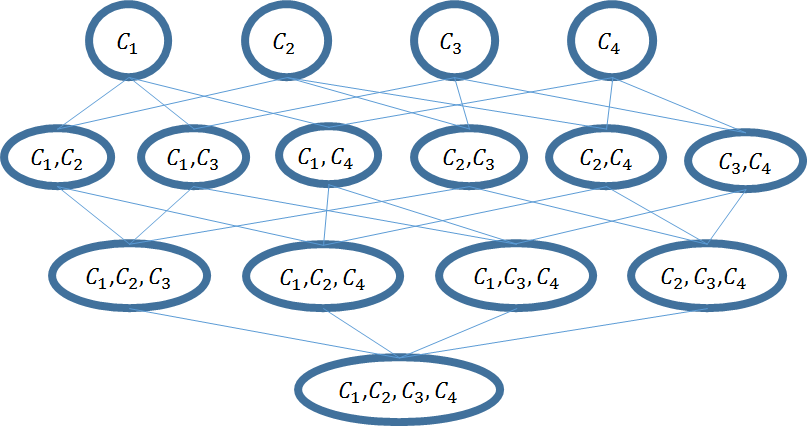
\includegraphics[width=0.75\columnwidth]{PowersetBasedSearch.png}%
\caption{An example of Powerset-Based search space of the minimal BRP wasted cost search problem.}%
\label{fig:power-search-space}%
\end{figure}

\begin{figure}%
\centering
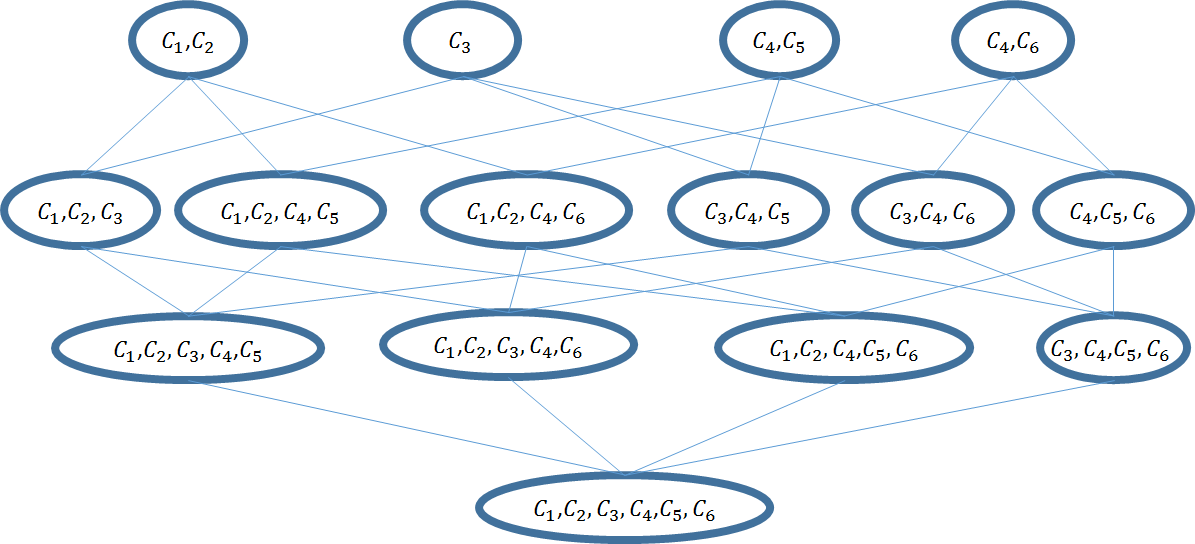
\includegraphics[width=0.85\columnwidth]{UnionBasedSearch.png}%
\caption{An example of Union-Based search space of the minimal BRP wasted cost search problem.}%
\label{fig:union-search-space}%
\end{figure}

As noted earlier, finding the best batch repair action according to the $k$-HP utility function is easy. 
This is not the case when using as a utility function 
one of the functions from the wasted effort family. 

\begin{definition}[Minimal BRP Wasted Cost Problem]
Given a BRP problem and a definition of $cost_{FN}$ and $cost_{FP}$, the minimal BRP wasted cost problem, denoted \brps{} is the problem of 
finding a subset of components $\gamma$ that minimizes $C_{WC}$. 
\end{definition}
Clearly, an optimal solution to \brps{} is a repair action that maximizes $U_{WC}$, since the goal is to minimize $C_{WC}$ and $U_{WC} = - C_{WC}$, as defined earlier .

In this section we discuss several search frameworks for solving the \brps{}.
%\meir{I dont remember if you defined formally our problem as a search problem, so if you did not do it this is the place to it. here you give an intuition and an example but in addition you should do it formally (nodes, operators etc.)}

%\roni{Wouldn't it be nice if you could prove that it's NP hard?}

%\begin{definition}[BRP as a search problem] Node $V$ defined as a subset of components $\gamma \subset COMPS$ to be repaired in a single batch repair action, where $\gamma$ is a subset of $COMPS$ that were not repaired yet. Edge $E$ represented by the pair $(V,{V}')$, if ${V}'$ is a direct child node of $V$ in the search space. Furthermore, an edge from node $V$ to ${V}'$, which defined by $\gamma$ and ${\gamma}'$ respectively, indicates that ${\gamma}'\subset\gamma$.  \end{definition} \roni{I don't see what we need this definition? what does it add over the previous definition of BRPS?  Hilla: I have added this definition because Meir requested for a formal definition of our problem as a search problem. I don't mind to remove it if you think its redundant} Roni: you already have a definition of it in the previous def.


\subsection{Search Space Choice}

%\roni{I don't understand. You already defined the state space, why are you doing it again? Put this sentence and the example at the beginning of the previous paragraph, and merge it. Ideally, you'll have two figures side-by-side, one with the powerset approach and the other with the union-based approach}

The basic approach defines the search space for the \brps{} problem, as a lattice of all possible subsets of components that were not repaired so far. Figure~\ref{fig:power-search-space} illustrates this search space for a system with four components, $C_1, C_2, C_3,$ and $C_4$. We call this approach of defining the search space as the all the possible subsets of components, as the {\em Powerset-Based Search}. 
An alternative approach, which we refer to as the {\em Union-Based Search}, is to consider the space of all possible unions of diagnoses. In this search space the root of the search is still an empty set of components, but the $i^{th}$ level of the search tree consists all subsets of components that are unions of $i$ diagnoses from $\Omega$. Thus, the first level in the tree is all subsets of components that form a diagnosis. Illustrated in Figure~\ref{fig:union-search-space} is an example of this Union-Based search space, of a system with six potential faulty components, $C_1, C_2, C_3, C_4, C_5$ and $C_6$, were the given set of four diagnoses are represented by the nodes in the first level of the search tree.
%; $\Omega_1={C_1,C_2}, \Omega_2={C_3}, \Omega_3={C_4,C_5}, \Omega_4={C_4,C_6}$.
The idea behind this approach has an intuitive reasoning that according to the known observation at least one of the diagnosis in $\Omega$ is supposed to be true. Thus, a repair action that does not repair all the components in at least one diagnosis cannot result in a fixed system. For example, if we look at the diagnoses of the case depicted in Figure~\ref{fig:union-search-space}; $\omega_1={C_1,C_2}, \omega_2={C_3}, \omega_3={C_4,C_5}, \omega_4={C_4,C_6}$. If the chosen repair action would have been for instance ${C_1}$, the system would not be fixed after repairing that component, and at least one more iteration of diagnosis, repair and testing would have to take place. That would be resulted with potentially higher total repair costs due to the $\cost_{repair}$.
%\roni{Consider adding a simple example of why repairing only part of a diagnosis is not sufficient}

%This search space formulation is referred to as the {\em Union-Based Search} while the former formulation described earlier is referred to as the {\em Powerset-Based Search}. 
To summarize the differences of the two presented search space formulation approaches; In {\em Powerset-Based Search} the children of a repair action $\gamma$ node will be formulated from all the possible sets components resulted by adding a single component to $\gamma$, while in {\em Union-Based Search} it would be from all of the possible sets components resulted by adding all the components in one diagnosis
%\roni{The above sentence is important, but is incorrect in terms of English. Please rephrase.}


%\meir{I would say: "There are two challenges by using a search approach for this problem: (1) A huge space search: for even medium sized systems with hundreds of components the search space becomes extremely very large. YOU SHOULD EVEN COMPUTE THE STATE SPACE. (2)  the second point will be that you mention in the next para.}

There are two challenges by using a search approach for BRP; First, dealing with a potentially huge search space, which for even medium sized systems with hundreds of components it becomes very large.
Another challenge regards to the monotonicity aspect of search spaces, as the \brps{} search space is not monotonic, as the cost of nodes along a path in the search space may increase or decrease~\cite{stern2014max}. 
That could come as a questionable statement, as the task in BRP as a search problem is to find the path which has the minimum cost. Usually this type of minimum-search problems has a monotonic search space, meaning there is no path that is better then any of its prefixes. In BRP monotonicity of the search space means that there is no set of components $(\gamma)$ which could be a better repair action then any of the set of components $(\gamma')$ such that ${\gamma}' \subset \gamma$. It is clear that the search space of BRP is not monotonic, as a superset of a repair action could easily be a better choice for a repair action. An easy example is to consider the case where the set of components $\gamma' \subset \omega$ is a partial diagnosis, and its superset $(\gamma)$, ${\gamma}' \subset {\gamma}$, contains all the components of a diagnosis $\omega \subseteq \gamma$. Repairing a partial diagnosis would require more repair actions, as the system would not be fixed for sure, while a repair action that contains all of the components of a diagnosis could be resulted with a fixed system.

%\roni{The reader does not know what a monotonic state space is and why it is important. Please explain (talk to me if you are not sure)} Hilla-done
Another way to clarify this point is to consider how the wasted cost changes along a path in the search space. 
Going along a path in the search space means considering larger sets of components to be repaired in a single batch repair action. This results in higher false positive costs, but also in lower false negative costs.
In other words, for every sets of components $\gamma' \subset \gamma$
it holds that $cost_{FN}(\gamma')\leq cost_{FN}(\gamma)$ 
and $cost_{FP}(\gamma')\geq cost_{FP}(\gamma)$. Since the wasted cost function is influenced both by $cost_{FP}$ and $cost_{FN}$, the wasted cost may increase or decrease. 
Having a non-monotonic search space affects the behavior of standard search algorithms~\cite{stern2014max}, as will be discussed below. 

\subsection{Uninformed Search}
The first search framework we present is a simple breadth-first search (BFS). 
In a monotonic search space, breadth-first search (and uniform-cost search in domains with non-unit edge costs) 
is guaranteed to find an optimal solution when a goal node is found. However, when the search space in non-monotonic an uninformed search like BFS guarantees an optimal solution only once all nodes in the search space have been explored. 
Therefore, to make the runtime manageable we limit the depth of the BFS, where the depth limit $k$ is a parameter. 
Thus, the search will explore the first $k$ levels of the search space, and return the batch repair set of components that has the highest wasted cost utility. 

\section{Heuristic Search}
An alternative classical heuristic search algorithm is the \astar{}~\cite{hart1968formal}. 
\astar{} implements a best-first search algorithmic framework. 
It maintains a list of open nodes (denoted OPEN), initialized by the root of the search tree. 
In every iteration it pops from OPEN the node $n$ with the lowest $f(n)=g(n)+h(n)$ value, 
where $g(n)$ is the cost spent so far for node $n$, and $h(n)$ is an admissible (lower bound) heuristic estimate of the lowest cost path from $n$ to a goal. Then, $n$ is {\em expanded}, which means that all its children (the nodes created by applying a single state-transition operator on $n$) 
are {\em generated} and inserted to OPEN.

In monotonic search spaces, the optimal solution is guaranteed once \astar{} expands the goal. 
%\meir{I comment the next sentences for the journal. You can uncomment them for the thesis.}
%This property allows joining two tasks that an optimal search algorithm needs to do: (1) find an optimal solution and (2) prove that it is optimal. 
% Stopping condition in non-monotone search spaces
%In non-monotonic search spaces, however, it is not possible to join these two tasks in the \astar{} framework. 
To find optimal solutions with \astar{} in non-monotonic search space one needs to keep track of the best solution it has found so far, referred to as the \emph{incumbent solution} and its cost is denoted as $C_{inc}$, as well as the lowest $f(n)$ value in OPEN, which is denoted by $f_{min}$. 
\footnote{Note that as the search progresses, the list of nodes in OPEN changes, and thus the lowest $f(n)$ value in OPEN may increase or decrease with the search. However, it is always a lower bound on the optimal solution, and therefore we denote by $f_{min}$ the highest of these values seen so far, to have the tightest lower bound observed so far.} 
The search halts when $C_{inc}\leq f_{min}$ and the optimal solution is guaranteed. 

To apply \astar{} for solving the \brps{} problem, one needs to define $g(n)$ and $h(n)$ for node $n$. 
This is not trivial in \brps{}, since there is no real notion of a path in the \brps{} search space. 
A node $n$ in the \brps{} search space represents a possible batch repair action. 
Denote $\comps[n]$ is the set of components intended to be repaired in batch repair action represented by node $n$. Then the cost of $n$ is simply the wasted cost of  this repair action, i.e., $C_{WC}(\comps[n])$. 
However, there is no clear definition of the cost of a path in this search space, and thus it is not clear what is the cost of reaching $n$ from the start ($g(n)$) or what is the cost of the lowest cost path from $n$ to a goal (which $h(n)$ should estimate). 

Alternatively, we define \astar{} slightly differently. 
Instead of the path-based $g(n)$ and $h(n)$, we use the following state-based values $cost(n)$ and $b_L(n)$, which are defined next.
$cost(n)$ corresponds to the cost of $n$, i.e., $C_{WC}(\comps[n])$. 
$b_L(n)$ is a heuristic function that estimates the cost of the lowest cost node in the subtree of the \brps{} search space that is rooted at $n$ (including $n$). 
We say that $b_L(n)$ is admissible if is a lower bound on the value it estimates: \begin{equation}
 b_L(n)\leq \min \{cost(n')| \comps[n]\subseteq \comps[n]\}  \label{eq:admissibility}
\end{equation}
Running \astar{} with $cost(n)$ and an admissible $b_L(n)$ is done as follows. In every iteration the node with the minimal $b_L(n)$ is expanded.
If $cost(n)$ is smaller than the incumbent solution then the incumbent solution is updated. The search continues until 
the cost of the incumbent solution is lower than or equal to the minimal $b_L(n)$ that is expanded. 
Proving that this \astar{} is equivalent to the traditional \astar{} definition that uses $g(n)$ and $h(n)$ is trivial, 
as it is easy to convert between $g(n)$ and $h(n)$, and $cost(n)$ and $b_L(n)$: 
$g(n)=cost(n)$ and $h(n)=b_l(n)-g(n)$. 
%\roni{do you mean here $b_l(n)$ or $b(n)$?}
However, it is more convenient to discuss costs and heuristics in state-based problems as \brps{} in terms of costs and heuristics over states, instead of paths. 

\subsection{Heuristics for BRP}
Now that we defined the heuristic function $b_L$ (Equation~\ref{eq:admissibility}), 
we present possible $b_L$ functions for \brps{}, based on the proposed versions of the wasted cost functions. 

Let $S(\gamma)$ denote the set of all supersets of $\gamma$, and let $S_i(\gamma)$ be a subset of $S(V)$ \meir{what is V? does it a subset of COMPS or of $\gamma$? you should mention it.} consisting all supersets of $V$ that have exactly $|V|+i$  components. From the search space perspective, 
for a node $n$ in the search tree we have that $S(\comps[n])$ is all the batch repair actions represented by nodes in the subtree  of the search space rooted by $n$, and $S_i(\comps[n])$ consists all batch repair actions represented by states in the $i^{th}$ level of the subtree rooted by $n$. 


We construct an admissible heuristic function for \brps{} by proposing a function $b_L(n,i)$ that bounds the cost of all states in $S_i(\comps[n])$. We call such functions a {\em $i$-level admissible} heuristic function. Then $b_L(n)$ would be the minimum over all
$i$-level admissible heuristic functions for any $i$. Formally, 
\begin{equation}
b_L(n)=\min_{i=[1,|\comps\setminus\comps[n]|]} b_L(n,i)
\label{eq:b-admissible}
\end{equation}
The value $|\comps\setminus\comps[n]|$ is the maximal number of levels under node $n$ in the search space, and we denote it by $m_n$.  
Note that for a bounded A* search, where the search is limited to a given depth, the maximal number of levels under node $n$ is determined according to the given bound.

\subsection{i-Level Admissible Heuristics}
The $i$-level admissible heuristic is composed of three components. A lower bound on the added false positive costs, an upper bound on the increase in system repair likelihood, and a lower bound on the added false negative costs. 

\noindent {\bf Bounding the false positive cost.} 
For a component $C$, let $c(C)$ be $(1-H(C))\cdot cost(C)$. 
To bound the false positive costs, we define $CL=\{c_1,\ldots,c_{m_n}\}$ as $c(C)$ values for every component $C$, sorted in ascending order, i.e., $c_1$ is the $c(\cdot)$ cost of the component with the lowest $c(\cdot)$ cost in $\comps\setminus\comps[n]$.  The sum $L_{fp}(n)=\sum_{j=1}^i c_i$ is a lower bound  on the false positive costs added to $cost(n)$ by any repair action in $S_i(\gamma)$.
Formally, 
\begin{multline}
\forall n'\in S_i(\comps[n])  : cost_{FP}(\comps[n])+ L_{fp}(n) \\
\leq cost_{FP}(\comps[n'])
\label{eq:fp-bound}
\end{multline}

\noindent {\bf Bounding the system repair likelihood.}
To bound the system repair likelihood, we define a second list, denoted $PL=\{p_1,\ldots, p_{m_n}\}$, which is used to estimate how much adding $i$ components will increase the probability the system will be repaired after the next batch repair action. To this end, we denote by $\Omega_{\hat{n}}$ the set of diagnoses that are not equal to or a subset of $\comps[n]$. If either of these diagnoses is correct then the system will not be repaired by the batch repair represented by $n$. We compute for every component $C$ that is not in $\comps[n]$ but is part of a  diagnosis in $\Omega_{\hat{n}}$ the sum of the probabilities of diagnoses in $\Omega_{\hat{n}}$ that contain it, i.e,. 
\[ p(C)=\sum_{\omega\in \Omega_{\hat{n}}\wedge C\in \omega} p(\omega) \]
The items in the $PL$ list are the $p(C)$ values for all component not in $\comps[n]$, 
sorted in descending order. I.e., $p_1$ is the component $C$ with the highest $p(C)$. 
The importance of the second list is that $U_{\sysrep{}}(n)=min(1, \sum_{j=1}^i p_i)$ is an upper bound on 
the increase to \sysrep{\comps[n]} that can be achieved by adding $i$ more components 
to $\comps[n]$. 

\begin{multline}
\forall n'\in S_i(\comps[n])  : \sysrep{\comps[n]}+\\ U_{\sysrep{}}(n) 
 \geq  \sysrep{\comps[n']}
\label{eq:sysrep-bound}
\end{multline}

\noindent {\bf Bounding the false negative costs.}
Bounding the false negative costs depend on the \brps{} variant. For the optimistic case, 
the false negative cost are always $cost_{repair}$. 
For the pessimistic case, we take a similar approach to that used to estimate the false positive costs: 
sort components in ascending order according to their $F(c)$ values and take the sum of the first $i^{th}$ components. Following the same reasoning as explained for bounding the false positive costs, this too is a lower bound on false negative costs added by in any node under $n$ over the false negative costs of $n$. 
Let $L^o_{fn}$ and $L^p_{fn}$ be the resulting lower bounds for the optimistic ($=cost_{repair}$) 
and pessimistic estimates of the false negative costs. We omit the superscript (``o''or ``p'') 
when it is not needed for exposition. 

Finally, we can define our $i$-level admissible heuristic as the summation of all three bounds, 
i.e., $b_L(n,i)=b(n)+L_{fp}+(-U_{\sysrep{}}(n))\cdot L_{fn}$. 

In order to ensure admissibility we offer an alternation for the presented $i$-level admissible heuristic,
i.e., $b_L(n,i)=b(n)+(-U_{\sysrep{}}(n))\cdot(L_{fn}-L_{fp})$. 
The alternative heuristic forgoes the additional false positive costs that could be added as a result of adding more components to the repair action. This change has been implicated in order to avoid double consideration in the false positive costs, thus, the false negative costs includes estimation of future repair actions. Furthermore, adding a component to the current repair action should be resulted with a change in the estimation of the false negative costs, thus that an additional component should not be considered as a future repair action and its costs need to be deducted from the false negative costs. That is the reason for subtracting the $L_{fp}$ from $L_{fn}$ in the alternative heuristic. 
It is easy to see that $b_L(n,i)$ is an $i$-level admissible heuristic, and consequently 
the $b_L$ heuristic given in Equation~\ref{eq:b-admissible} is admissible. \meir{dont we need to prove?}

%bounded fval

\section{Local Search}
Finally, we also consider a simple local search approach. 
Specifically, we propose Hill Climbing search, where in every iteration we consider adding a single component to the batch repair action. All possible components are considered, and the wasted cost of the resulting 
batch repair action is computed. If there exists a single component that can be added and that will result in decreasing the wasted cost, then the component that decreases the wasted cost the most is chosen. 
If no such component exists, then we return the current batch repair action. 


There are many other, more sophisticated, local search algorithms~\cite{lourencco2003iterated}. Techniques such as random restarts, simulated annealing, Tabu search~\cite{glover2013tabu}, and others have been shown to be very effective in many domains. Similarly, there are more sophisticated optimal heuristic search algorithm including Enhanced Partial Expansion A*~\cite{goldenberg2014enanced}, IDA*~\cite{korf1985depth}, and RBFS~\cite{korf1993linear}, as well as a variety of bounded suboptimal search algorithms. However, the goal of this work is not to perform a comprehensive comparison of different search paradigms, but to demonstrate their potential use in solving the BRP problem. 

\chapter{BRP as a Planning Problem}
%An alternative approach to address BRP considers it as a planning under uncertainty problem, model it as a Markov Decision Process (MDP) and solve it appropriately. 

The second approach we propose for solving BRP, models it as a Stochastic Shortest Path Markov Decision Process (SSP-MDP)~\cite{bertsekas1995dynamic}. An SSP-MDP is a common model for planning problems where actions may have stochastic outcomes, and the task is to reach a goal state with minimal expected cost. 
In BRP, repair actions have stochastic outcomes -- the system is either fixed or not. Following the maximum expected utility principle, we aim at minimizing the expected total repair cost. %This approach can be viewed as a variant of decision theoretic troubleshooting (DTT) [1]. See Section 7 for a discusses on the difference and similarity between our proposed approach to BRP and DTT.

Formally, an SSP-MDP is defined by a tuple $\left \langle S, A,Tr,R,I,G \right \rangle$ where $S$ and $A$ are the sets of states and actions respectively. $Tr(s,a,{s}')$ is the transition function, returning the probability that performing action $a$ at state $s$ leads to state ${s}'$. $R(s,a)$ is the reward of performing an action $a$ at state $s$. $I$ is the initial states and $G$ is the set of terminal states.

In our case, states are the \emph{system states} during a repair process and actions are the \emph{repair actions}, which defined earlier. The reward of performing an action is minus the cost of the corresponding repair action, $-cost(Repair(a))$. The possible outcomes of an action are that the system is fixed or not. The probability of each outcome is given by $SysRepair(a)$. An outcome where the system is fixed corresponds to a goal state.
Consider the other outcome, where the system is not fixed. In such a case, the components in repair action $a$ are added to the set of repaired components, 
and removed from the set of diagnoses. For example, 
if the set of diagnoses contains two diagnoses $\{A,B\}$
 $\{A,C\}$ and we repaired $A$, then the remaining set of diagnoses is $\{B\}$ and $\{C\}$. 
 Note that in some cases a new observation is obtained at this stage, in which case the diagnosis algorithm needs to be re-run using the new observation, to generate more refined diagnoses. 
 
 
 Formalizing BRP as a SSP-MDP is useful because it allows using SSP-MDP solvers to compute the best (batch) repair action to perform. We elaborated on this next. 
 
\section{Using Baseline MDP Solvers}
\meir{i think a visual example will help to follow this section too.}

Baseline SSP-MDP solvers such as Value Iteration require iterating over the entire state space in order to compute the optimal solution. 
Such approaches are no feasible, since in our case the state space of the SSP-MDP is too large to be solved optimally in practice. 

To see this, observe that the set of possible actions in a state is exponential in $|\overline{Repaired}|$, as every subset of $\overline{Repaired}$ can be a repair action. Also, the number of states that can be reached after applying an action is also potentially exponential in the number of components. This is because when a repair action fails, the number of possible observations is at most equal to the number of diagnoses that are not fixed by the past repair actions. The number of such diagnoses can be exponential in the number of system components.
%Also, the number of states that can be reached after applying an action is also potentially exponential in the number of system outputs. This is because when a repair action fails, the number of possible observations is at most equal to the number of diagnoses that are not fixed by the past repair actions. The number of such diagnoses can be exponential in the number of system components, but the number of different outputs is at most exponential in the number of system outputs. 
%\roni{The above discussion on the number of states is not very clear.}

The state space described by our MDP is thus too large to be solve optimally using baseline SSP-MDP solvers. 
Therefore, we implemented an algorithm that is specifically designed for our state space.



\section{UCT Based Implementation}
The specific algorithm we implemented is the Upper bound Confidence for Tree (UCT)~\cite{kocsis2006bandit} algorithm. UCT has been applied successfully to solve  games and planning problems. We provide here a brief description of our UCT implementation. 
UCT is designed to explore the MDP state space in a manner that balances \emph{exploration} and \emph{exploitation}, that is, it balances between exploring the outcome of actions not considered so far, and exploiting the knowledge gained so far about the state space and choose the best batch repair action. 


In every iteration of UCT, the algorithm explores a trajectory (a sequence of action and possible outcome) in the state space starting from the initial state and moving from one system state to the next by choosing a (batch) repair action. UCT uses the UCB (Upper Confidence Bounds) rule~\cite{auer2002finite} to choose an action in each tree node. 

\subsection{The UCB Rule}
The UCB rule requires maintaining for every explored state the number of times each state has been visited, denoted $NB_{s}$, as well as the number of times a specific action was taken in a specific state, denoted $NB_{s,a}$. In addition, UCB requires to store a state-action vector $Q(s,a)$ that contains the average seen cost (reward) of taking action $a$ when in state $s$. 

%In every iteration of the algorithm it starts descending from the initial state by choosing a repair action and moving from one system state to the next. %The transition between the states is done as follows: The set of diagnoses is derived from the observation and the knowledge about which components have been repaired, which defines the current system state, officiate as the possible (repair) actions to be taken in a currently visited state\meir{the explanation of the action is not clear. Also, you try to explain here what are states and actions, which is not limited to UCT. You should formalize it when presenting the MDP model.}. 
UCB choses the action that maximizes the following utility function:
\begin{equation}
U_s(a)= Q(s,a) + \alpha\cdot \sqrt{\frac{ln(NB_{s})}{NB_{s,a}}}
\label{eq:ucb}
\end{equation}
where $\alpha$ is a parameter. In our implementation, we set $\alpha$ to be the number of diagnoses in the initial state. We experimented with other possible values of $\alpha$ and found this to be the most effective in the experiments we performed.


Note that for actions that have not been chosen yet, $NB_{s,a} = 0$, which results in a division by zero in the UCB formula (Eq.~\ref{eq:ucb}). To resolve this, we define an alternative utility function $U_s(a)_0$ for 
actions that have not been chosen yet: 
\[ U_s(a)_0 = - \frac{cost_{FP}}{|a|} \]
Here too we explore several alternatives for 
such a \emph{default} utility function and found that the above worked well.

\subsection{Value Propagation}

In UCT, the values of the state-action vector $Q(s,a)$ for every state-action pair in the chosen trajectory needs to be updated. This is done in a bottom up, i.e., starting from the last state-action pair in the chosen trajectory. To control the running time of our UCT implementation, we limited the depth of the trajectory in each iteration, where this limit is a parameter denoted by $LH$. 


Thus, the last state in a chosen trajectory 
can be either a goal, i.e., when the system is fixed, or 
a state at depth $LH$. In case the final state is a goal state, which means that the system is fixed, the propagated value is initialized with 0. If the final state is not a goal state, which means that  depth $LH$ has been reached, the value of state $s$ is defined as follow: 
$cost(a)=\sum_{c\in \overline{Repaired}} F(c)\cdot(cost_{repair}+cost(c))$
where $\overline{Repaired} \in s$ is the set of components that have not been repaired yet, as defined in Section \ref{sec:Repair_Likelihood}. 

Next, each state-action pair value $Q(s,a)$ is updated by accumulating the received values propagated from the lower levels of the trajectory, together with its immediate reward, $R(s,a) = cost(Repair(a))$, and the resulted value is passed on to the level above. 

The number UCT iterations we run is a parameter. After completing the requested amount of iterations, the repair action eventually chosen is the one with the highest state-action value over all the state-actions pairs in the initial state.

\chapter{Experimental Results}

\begin{figure}{}%{4cm}
\begin{center}
  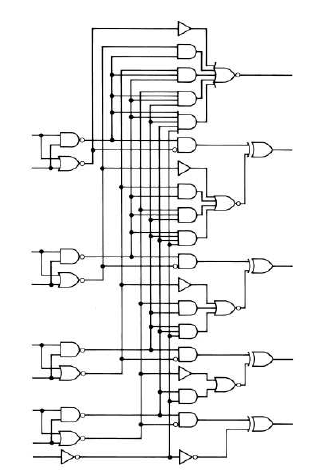
\includegraphics[width=0.5\columnwidth]{74283.png}
  \caption{A logic diagram of ISCAS 74283 4-bit adder.}
  \label{fig:74283}
\end{center}
\end{figure}

%ISCAS
We evaluated the proposed BRP algorithms on two different benchmarks. The first is the standard ISCAS 85~\cite{Brglez89} and 74XXX benchmarks~\cite{Hansen99}, which represents Boolean circuit systems. Figure \ref{fig:74283} presents a logic diagram of one of these systems called 74283, which is a 4-bit adder. $\COMPS$ in this benchmark domain are the Boolean gates. $\SD$ is the behavior description of the components, for instance, the healthy behavior of an $\textit{OR}$ gate is the logical OR operation, while abnormal behaviors can be stuck at 1, stuck at 0, or flip (i.e., outputting the opposite of the normal output).  $\OBS$ is an observation of the inputs and outputs values of the system. A diagnosis states which gates are healthy and which are in a faulty mode. 
Our BRP algorithms output a set of gates to fix. 

\begin{table}\centering
{\small
\begin{tabular}{|l|r|r|r|r|}
\hline
 {\bf Name} & {\bf $|${\tiny \COMPS}$|$} & {\bf in} & {\bf out} & {\bf \#observations} \\
\hline
    74182  & 19    & 9    & 5    & 25 \\
    74283  & 36    & 9    & 5    & 22 \\
\hline
    c432   & 160   & 36   & 7    & 23\\
    c880   & 383   & 60   & 26   &  30\\
\hline
\end{tabular}
\caption{The Benchmark suite: systems  {\small 74XXX} and
         {\small ISCAS-85}, and scenarios Feldman.}
\label{tab:systems}
}
\end{table}%


Details of the standard Boolean circuits we used in our experiments are presented in Table \ref{tab:systems}. The systems {\small 74XXX}~\cite{Hansen99} are described in the first three rows, and additional three systems of {\small ISCAS-85} \cite{Brglez89} are described in the following three rows. Observations were selected randomly from Feldman et al.'s~\shortcite{feldman2010approximate} known benchmark of observations.

%Physiotherapy
The second domain we experimented on is from the medical physiotherapy field. The data used in our experiments was obtained from simulations of medical physiotherapy cases of human patients. In total, we have received more then 500 observation to experiment on. 


% add reference to the physiotherapy work
% add figure of physiotherapy case

%parameters - prior probability and costs
In both domains, we set the prior probability of each gate to be faulty to 0.01 and chose a single diagnosis for each observation to serve as the real injected faults. This is needed to decide when the system is fixed. Note that this ``true'' diagnosis was chosen with probability proportional to its likelihood of being correct, computed according to the priors mentioned above under the standard assumption of fault independence. The component repair cost was set to 5, and we experimented with repair overhead ($cost_{repair}$) costs of 5, 10, 15, 20, and 25.

Some of the evaluated algorithms require predetermined parameters. In particular, some of the search-based algorithms had a \emph{bound} parameter that specifies the maximal number of diagnoses to consider repairing (the union of their components). Our UCT implementation also required parameters: the lookahead depth ($LH$) 
and the number of iteration. 
After some parameter tuning, we used a bound of up to 3 for the search algorithms, and $LH=5$ and 10,000 iterations for our UCT. 


%diagnoses generation and cardinality:
For every observation, we computed the a set of corresponding diagnoses. In the physiotherapy domain we considered all the subset minimal diagnoses.  
In the Boolean circuits domain we further limited the set of diagnoses to only the minimal cardinality diagnoses, since the set of all subset minimal diagnoses was too large. 


In every experiment we run the evaluated algorithm to choose a batch repair action. Then performed this repair action. If the system is not fixed yet, then we run again the evaluated algorithm to choose the next batch repair action. This process continues until the system is fixed. The overall costs spent during this process is recorded. We limited the runtime of all algorithm to 5 minutes. 
An algorithm that reached this timeout was forced to return the best repair action is found so far. 



In addition, we ran another set of experiments on a chosen portion of the obtained data, which included only the observation in which the matching set of diagnoses size did not exceed 30 diagnoses. That is because the computation complexity depends mostly in the size of the given set of diagnoses, and by adding the mentioned restriction criterion for the experimented cases we can reduce the number of times the algorithms will reach the timeout limitation, and by that increases the percentage of cases in which the optimal solution was returned. 

\section{Evaluated Algorithms}

%\roni{Here list all the algorithms you have in your experiments.} %hilla- done
We have experimented on our purposed BRP algorithms; The search- based algorithms with different objective functions: Hill Climbing, A*-Powerset, A*-Union and UnionK, As well as the MDP based algorithm and some baseline algorithms:K-HP and BD-Batch. 

The main hypothesis of this line of work is that performing batch repair actions can save repair costs, compared to only performing repair actions that repair a single component. Thus, we compared our BRP algorithms to 1-HP, in which the component that is most likely to be faulty is repaired. A similar approach was used by previous work on test planning~\cite{zamir2014using}. Another baseline repair algorithm we evaluated experimentally is to repair all components of the most likely diagnosis in a single batch repair action denoted {\em Batch Best Diagnosis} (hereinafter, BD-batch).

\section{Results}

%results tables:
\begin{table}[]
\centering
\caption{Experiments results on Physiotherapy cases: Average repair costs until the system is fixed}
\label{tab:physioRes}
\begin{tabular}{|l|l|l|l|l|l|l|}
\hline
\multicolumn{2}{|l|}{}                                                          & \multicolumn{5}{c|}{\textbf{Overhead Cost}}                        \\ \hline
\textbf{Planner}                                           & \textbf{Algorithm} & \textbf{5} & \textbf{10} & \textbf{15} & \textbf{20} & \textbf{25} \\ \hline
Single Component                                           & KHigestProb\_1     & 31.9       & 47.9        & 63.8        & 79.8        & 95.7        \\ \hline
Baseline                                                   & BatchBestDiagnosis & 29.9       & 44.4        & 58.8        & 73.3        & 87.8        \\ \hline
Baseline                                                   & KHigestProb\_2     & 27.8       & 37.2        & 46.5        & 55.9        & 65.2        \\ \hline
Baseline                                                   & KHigestProb\_3     & 28.9       & 36.2        & 43.6        & 51.0        & 58.3        \\ \hline
\begin{tabular}[c]{@{}l@{}}Batch\\   bound-1\end{tabular}  & A*\_Union       & 29.3       & 42.0        & 55.1        & 67.7        & 81.2        \\ \hline
Batch bound-1                                              & HillClimbing       & 29.3       & 42.0        & 55.1        & 67.7        & 81.2        \\ \hline
Batch bound-1                                              & MDP                & 27.3       & 40.6        & 54.8        & 67.3        & 77.5        \\ \hline
Batch bound-1                                              & UnionK             & 29.3       & 41.9        & 55.2        & 67.6        & 81.2        \\ \hline
\begin{tabular}[c]{@{}l@{}}Batch\\   bound-2\end{tabular}  & A*\_Union       & 26.4       & 34.2        & 42.5        & 50.6        & 58.9        \\ \hline
Batch bound-2                                              & HillClimbing       & 26.7       & 34.4        & 42.5        & 50.6        & 58.8        \\ \hline
Batch bound-2                                              & MDP                & 26.0       & 33.6        & 41.2        & 51.2        & 59.1        \\ \hline
Batch bound-2                                              & UnionK             & 26.4       & 34.5        & 42.2        & 51.0        & 58.5        \\ \hline
\begin{tabular}[c]{@{}l@{}}Batch\\   bound-3\end{tabular}  & A*\_Union       & \textbf{25.7}      & 31.8        & 39.1        & 45.4        & 51.4        \\ \hline
Batch bound-3                                              & HillClimbing       & 25.9       & 32.4        & 39.4        & 45.8        & 52.4        \\ \hline
Batch bound-3                                              & MDP                & 26.8       & 32.6        & 39.8        & 46.2        & 50.8        \\ \hline
Batch bound-3                                              & UnionK             & \textbf{25.7}       & 32.2        & 38.4        & 44.8        & 51.8        \\ \hline
\begin{tabular}[c]{@{}l@{}}Batch\\   ubounded\end{tabular} & A*\_PowerSet    & 26.0       & \textbf{31.4}       & \textbf{37.3}       & \textbf{43.1}        & \textbf{48.0}        \\ \hline
Batch ubounded                                             & A*\_Union       & 25.9       & \textbf{31.5}        & \textbf{37.5}       & \textbf{43.0}        & \textbf{48.1}       \\ \hline
Batch ubounded                                             & HillClimbing       & 25.9       & 32.0        & 37.9        & 43.4        & \textbf{48.2}        \\ \hline
\end{tabular}
\end{table}

\begin{table}[]
\centering
\caption{Experiments results on ISCAS systems 74182 and 74283: Average repair costs until the system is fixed}
\label{tab:ISCASRes_7}
\resizebox{\textwidth}{!}{%
\begin{tabular}{|l|l|c|c|c|c|c|c|c|c|c|c|}
\hline
\multicolumn{2}{|l|}{\textbf{System}}                                           & \multicolumn{5}{c|}{\textbf{74182}}                                 & \multicolumn{5}{c|}{\textbf{74283}}                                 \\ \hline
\textbf{Planner}                                           & \textbf{Algorithm} & \textbf{5} & \textbf{10} & \textbf{15} & \textbf{20} & \textbf{25} & \textbf{5} & \textbf{10} & \textbf{15} & \textbf{20} & \textbf{25} \\ \hline
Single Component                                           & KHigestProb\_1     & 47.4       & 71.2        & 94.9        & 118.6       & 142.3       & 40.5       & 60.7        & 80.9        & 101.1       & 121.4       \\ \hline
Baseline                                                   & BatchBestDiagnosis & 35.7       & 49.0        & 62.3        & 75.5        & 88.8        & 37.6       & 53.8        & 69.9        & 86.1        & 102.2       \\ \hline
Baseline                                                   & KHigestProb\_2     & 40.0       & 53.6        & 67.2        & 80.8        & 94.5        & 35.7       & 47.8        & 59.8        & 71.9        & 84.0        \\ \hline
Baseline                                                   & KHigestProb\_3     & 38.2       & 48.3        & 58.3        & 68.3        & 78.3        & 35.5       & 44.8        & 54.1        & 63.4        & 72.8        \\ \hline
\begin{tabular}[c]{@{}l@{}}Batch\\   bound-1\end{tabular}  & A*\_Union       & 35.6       & 49.5        & 63.2        & 77.0        & 89.3        & 36.9       & 53.0        & 68.7        & 84.9        & 101.8       \\ \hline
Batch bound-1                                              & HillClimbing       & 35.6       & 49.5        & 63.2        & 77.0        & 89.3        & 36.9       & 53.0        & 68.7        & 84.9        & 101.8       \\ \hline
Batch bound-1                                              & MDP                & 37.3       & 49.8        & 67.4        & 75.2        & 92.2        & 36.8       & 49.8        & 63.3        & 90.4        & 101.0       \\ \hline
Batch bound-1                                              & UnionK             & 35.7       & 49.6        & 63.2        & 77.0        & 89.3        & 36.9       & 53.0        & 68.7        & 84.9        & 101.8       \\ \hline
\begin{tabular}[c]{@{}l@{}}Batch\\   bound-2\end{tabular}  & A*\_Union       & \textbf{33.8}       & \textbf{41.6}        & 50.3        & 57.8        & 66.2        & 33.9       & 43.4        & 53.2        & 61.7        & 72.2        \\ \hline
Batch bound-2                                              & HillClimbing       & 34.0       & 42.4        & 50.6        & 58.7        & 66.2        & \textbf{33.2}       & 43.2        & 52.9        & 60.9        & 71.9        \\ \hline
Batch bound-2                                              & MDP                & 35.0       & 42.2        & 52.0        & 59.9        & 69.1        & 34.7       & 42.4        & 51.2        & 62.6        & 73.1        \\ \hline
Batch bound-2                                              & UnionK             & \textbf{33.8}       & \textbf{41.2}        & 49.6        & 57.2        & 65.9        & 33.9       & 43.2        & 53.3        & 62.1        & 72.2        \\ \hline
\begin{tabular}[c]{@{}l@{}}Batch\\   bound-3\end{tabular}  & A*\_Union       & 35.1       & \textbf{41.4}        & 47.9        & 54.6        & 60.9        & 33.8       & 42.0        & 49.8        & 56.7        & 64.0        \\ \hline
Batch bound-3                                              & HillClimbing       & 34.9       & 41.7        & \textbf{47.6}        & \textbf{53.8}        & 60.3        & 34.0       & 41.7        & 49.5        & 55.9        & 63.9        \\ \hline
Batch bound-3                                              & MDP                & 35.4       & \textbf{41.6}        & 49.2        & 55.2        & 61.7        & 34.6       & \textbf{41.3}        & \textbf{48.0}        & 58.4        & 61.7        \\ \hline
Batch bound-3                                              & UnionK             & 34.8       & \textbf{41.4}        & \textbf{47.6}        & 54.4        & 60.8        & \textbf{33.0}       & \textbf{41.4}        & 49.2        & 57.5        & 64.7        \\ \hline
\begin{tabular}[c]{@{}l@{}}Batch\\   ubounded\end{tabular} & A*\_PowerSet    & 35.3       & 42.0        & 48.6        & 54.1        & \textbf{59.1}        & 34.4       & 41.8        & 48.7        & \textbf{54.8}        & 60.2        \\ \hline
Batch ubounded                                             & A*\_Union       & 35.4       & 41.8        & 48.4        & \textbf{53.8}       & \textbf{59.1}        & 34.6       & 42.5        & 49.1        & \textbf{55.0}        & 60.3        \\ \hline
Batch ubounded                                             & HillClimbing       & 35.4       & 42.6        & 48.5        & 54.0        & \textbf{59.1}        & 34.7       & 42.1        & 48.9        & \textbf{54.9}        & \textbf{59.7}        \\ \hline
\end{tabular}%
}
\end{table}


\begin{table}[]
\centering
\caption{Experiments results on ISCAS systems C432 and C880: Average repair costs until the system is fixed}
\label{tab:ISCASRes_C}
\resizebox{\textwidth}{!}{%
\begin{tabular}{|l|l|c|c|c|c|c|c|c|c|c|c|}
\hline
\multicolumn{2}{|l|}{\textbf{System}}                                           & \multicolumn{5}{c|}{\textbf{c432}}                                 & \multicolumn{5}{c|}{\textbf{c880}}                                 \\ \hline
\textbf{Planner}                                           & \textbf{Algorithm} & \textbf{5} & \textbf{10} & \textbf{15} & \textbf{20} & \textbf{25} & \textbf{5} & \textbf{10} & \textbf{15} & \textbf{20} & \textbf{25} \\ \hline
Single Component                                           & KHigestProb\_1     & 47.9       & 71.8        & 95.7        & 119.7       & 143.6       & 43.2       & 64.7        & 86.3        & 107.9       & 129.5       \\ \hline
Baseline                                                   & BatchBestDiagnosis & 44.8       & 62.7        & 80.6        & 98.6        & 116.5       & 41.2       & 59.5        & 77.7        & 96.0        & 114.2       \\ \hline
Baseline                                                   & KHigestProb\_2     & 42.6       & 57.0        & 71.4        & 85.8        & 100.3       & 37.8       & 50.5        & 63.3        & 76.1        & 88.9        \\ \hline
Baseline                                                   & KHigestProb\_3     & 40.8       & 51.4        & 62.0        & 72.6        & 83.2        & 36.3       & 45.9        & 55.5        & 65.1        & 74.7        \\ \hline
\begin{tabular}[c]{@{}l@{}}Batch\\   bound-1\end{tabular}  & A*\_Union       & 43.9       & 61.5        & 78.7        & 97.9        & 116.2       & 40.4       & 58.4        & 76.3        & 94.8        & 113.9       \\ \hline
Batch bound-1                                              & HillClimbing       & 43.9       & 61.5        & 78.7        & 97.9        & 116.2       & 40.4       & 58.4        & 76.3        & 94.8        & 113.9       \\ \hline
Batch bound-1                                              & MDP                & 45.8       & 59.8        & 78.5        & 94.8        & 112.4       & 40.1       & 47.4        & 77.8        & 100.4       & 110.6       \\ \hline
Batch bound-1                                              & UnionK             & 43.9       & 61.5        & 78.7        & 97.9        & 116.2       & 40.4       & 58.4        & 76.3        & 94.8        & 113.9       \\ \hline
\begin{tabular}[c]{@{}l@{}}Batch\\   bound-2\end{tabular}  & A*\_Union       & 41.1       & 52.2        & 62.3        & 73.0        & 84.4        & 36.4       & 47.2        & 57.4        & 68.4        & 79.2        \\ \hline
Batch bound-2                                              & HillClimbing       & 40.6       & 51.1        & 61.6        & 72.0        & 83.2        & 36.3       & 47.0        & 57.4        & 68.4        & 79.2        \\ \hline
Batch bound-2                                              & MDP                & 40.6       & 49.7        & 62.8        & 75.5        & 81.6        & 35.9       & 46.7        & 58.8        & 62.2        & 82.0        \\ \hline
Batch bound-2                                              & UnionK             & 40.7       & 52.2        & 63.0        & 73.6        & 84.0        & 36.7       & 47.9        & 59.1        & 68.6        & 78.9        \\ \hline
\begin{tabular}[c]{@{}l@{}}Batch\\   bound-3\end{tabular}  & A*\_Union       & 41.1       & 49.4        & 57.6        & 65.9        & 73.8        & 35.9       & 44.5        & 50.8        & 59.3        & 66.6        \\ \hline
Batch bound-3                                              & HillClimbing       & 40.1       & 48.7        & 56.8        & 65.2        & 73.2        & 35.6       & 44.6        & 50.9        & 59.1        & 66.6        \\ \hline
Batch bound-3                                              & MDP                & \textbf{39.9}       & 50.3        & 57.0        & 64.2        & 72.4        & \textbf{33.9}       & \textbf{41.5}        & 52.7        & 59.7        & 64.7        \\ \hline
Batch bound-3                                              & UnionK             & 40.9       & 49.1        & 57.5        & 64.9        & 72.9        & 35.3       & 43.8        & 50.5        & 59.1        & 66.7        \\ \hline
\begin{tabular}[c]{@{}l@{}}Batch\\   ubounded\end{tabular} & A*\_PowerSet    & 42.3       & \textbf{47.9}        & \textbf{55.5}        & 63.1        & 70.2        & 35.2       & 43.1        & \textbf{47.4}        & \textbf{52.3}        & 58.5        \\ \hline
Batch ubounded                                             & A*\_Union       & 43.0       & 48.7        & \textbf{55.5}        & \textbf{61.6}        & \textbf{67.4}        & 35.1       & \textbf{41.6}        & 48.0        & 52.8        & \textbf{57.9}        \\ \hline
Batch ubounded                                             & HillClimbing       & 42.2       & 49.4        & 56.0        & 62.4        & 67.7        & 35.7       & 43.3        & 48.4        & 53.1        & 59.2        \\ \hline
\end{tabular}%
}
\end{table}


%\roni{In all experiments, you first describe the results, and only then talk about trends. So, what you need here is a paragraph of this form: ``Table X shows the average troubleshooting costs incured in our experiments on the Y domain for the different BRP algorithms. Column ``Planner'' refers to ....Column ``Algorithm'' refers to. The columns ``5'', ``10'', ``15'', ``20'', and ``25'' show the overhead costs. In every column we highlighted in bold the best performing algorithm. [[Roni: you really should do this]]'' Obviously, fill in the X and Y and ... above} 
%\hilla{done}

Table ~\ref{tab:physioRes} shows the average troubleshooting costs incurred in our experiments on the physiotherapy domain for the different repair algorithms. Column ``Algorithm'' refers to the algorithm that was used, and column ``Planner'' refers to the type of repair planner that the algorithm defines. The columns ``5'', ``10'', ``15'', ``20'', and ``25'' show the overhead costs. In every column we highlighted in bold the best performing algorithm. Tables ~\ref{tab:ISCASRes_7} and ~\ref{tab:ISCASRes_C}, which structured in the same format as table ~\ref{tab:physioRes}, show the average troubleshooting costs incurred in our experiments on the ISCAS domain.

%1-single vs batch results:
The first trend we highlight is that in all cases, using a BRP algorithm that can choose a batch repair action resulted in significantly less costs compared to the 1-HP, in which a single component is repaired in each round. 

%\roni{Every time you talk about a trend, you need to provide a concrete example. So you should add here a text like this:``For example, algorithm X for system Y and overhead Z required W cost on average while 1-HP on the same setting required K''  (of course, choose a place where W is larger than K)} 
%hilla-done

For example, in the experimental results of the physiotherapy domain, algorithm A*-Union and overhead 20 required cost of 43 on average, while 1-HP on the same setting required 79.8 which is almost twice as much.
Another good example from the ISCAS domain results of system 74182, where all the unbounded batch repair algorithms required on average a total cost of 59.1, when the overhead cost was set to 25, while the 1-HP with the same overhead required 142.3.
Additional charts of the results are presented in order to demonstrate this trends visually; Figures ~\ref{fig:P-all-graph}, ~\ref{fig:I-batch-base-single} and ~\ref{fig:I-bvs-74182} plots the overhead cost on the X-axis and the average repair cost on the Y-axis.

%\roni{Here too. First explain the figures: ``Figure A plots B on the X-axis and C on the Y-axis. hilla-done
%''Also, does the figures provide additional information over the tables above? if so - say thisif not, then choose either the table or the figure. My recommendation: go for the figures, and throw the table to an appendix. } 

This results supports our main claim that reasoning about the possibility of batch repair is important. 
As shown in Figure~\ref{fig:I-bvs-74182} and Figure~\ref{fig:P-all-graph}, increasing the repair overhead causes all algorithms to require more cost to fix the system. However, the advantage of batch repair algorithms over 1-HP increase as repair overhead costs increases, demonstrating that the importance of batch repair is greater when overhead costs are higher. 
%\roni{Good paragraph}

\begin{figure}{}
\frame{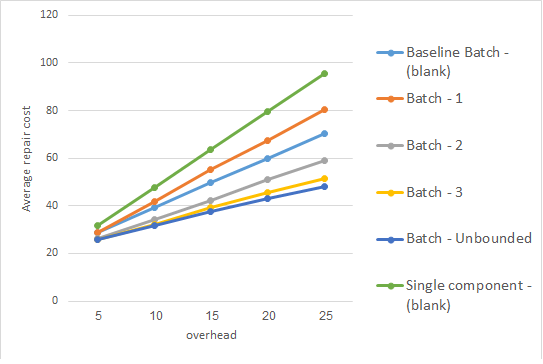
\includegraphics[width=0.8\columnwidth]{Charts/P_batch_base_single_graph.png}}
  \caption{Average repair costs of physiotherapy cases experimental results using batch (bounded and unbounded), baseline and single component repair algorithms, with different overheads.}
  \label{fig:P-all-graph}
\end{figure}

\begin{figure}{}
\frame{\includegraphics[width=0.8\columnwidth]{Charts/I_batch_base_single.png}}
  \caption{Average repair costs experimental results on ISCAS systems,
  %\roni{Go over the entire paper and verify you use ISCAS, not Iscas. It is an acronym so all letters should be capitalized}  \hilla{done}
  using search based batch repair algorithms, A*-Union and Hill Climbing, vs baseline and single component repair algorithms with overhead of 25.}
  \label{fig:I-batch-base-single}
\end{figure}

\begin{figure}{}
\frame{\includegraphics[width=0.8\columnwidth]{Charts/I_bvs_74182.png}}
  \caption{Average repair costs of ISCAS system 74182 experimental results, using single and batch repair algorithms with different overheads.}
  \label{fig:I-bvs-74182}
\end{figure}

\subsection{Comparison of Batch Repair Algorithms}
%2-batch algos vs base
Next, we compared the performance of our search-based BRP algorithms and our UCT-based BRP algorithm
against the baseline algorithms, K-HP and BD-Batch.
In Figure~\ref{fig:P-batch-base}, Figure~\ref{fig:I-batch-base-single} and ~\ref{fig:P-BD-UK} plots the overhead cost on the X-axis and the average repair cost on the Y-axis. We can see in those charts the large gap between the A*-Powerset algorithm to the rest, which grows more and more as the overhead grows. 

%\roni{I see the figures still rely on colors and not on shapes or texture. Don't change it now for your thesis but for the journal this will be needed}

The results in Figure~\ref{fig:P-BD-UK} show the benefit our our WC utility function compared to the simpler BD-Batch algorithm. The results show a clear advantage of our Union-based search algorithms even when limiting it to bound 1. 
%\roni{As above, choose a specific data point to mention that demonstrates the trend}. %hilla-done
For example, in the experimental results of the physiotherapy domain, Union-based search algorithm and overhead 20 required cost of 67.6 on average, while BD-Batch on the same setting required 73.3.

These results highlight the benefit of our proposed utility functions for evaluating a repair action candidate. That is because the difference between BD-Batch and Union-based search with bound 1 is that BD chooses the diagnosis to repair according to its probability to be correct and not according to our WC utility function. 

\begin{figure}{}
\frame{\includegraphics[width=0.8\columnwidth]{Charts/P_batch_base.png}}
  \caption{Average repair costs of physiotherapy cases experimental results using A*-Powerset based batch repair algorithm, vs using the baseline algorithms with different overheads.}
  \label{fig:P-batch-base}
\end{figure}

\begin{figure}{}
\frame{\includegraphics[width=0.8\columnwidth]{Charts/P_BDvsUK.png}}
  \caption{Average repair costs of physiotherapy cases experimental results Union-1 vs BD with different overheads.}
  \label{fig:P-BD-UK}
\end{figure}

\begin{figure}{}
\frame{\includegraphics[width=0.8\columnwidth]{Charts/P_obj_o_15.png}}
  \caption{Total average repair costs of experimental results with overhead = 15 over the Physiotherapy cases, of all the search based batch repair algorithms with overhead of 15. Presents comparison of three versions of utility function which estimated the wasted cost of a repair action candidates}
  \label{fig:P-obj-15}
\end{figure}

%3-Objective functions
\subsection{Comparison of WC Utility Functions}
Figure~\ref{fig:P-obj-15} presents the significant differences between the results of the three versions our proposed WC utility function. The x-axis represents the different bounds of the search algorithms and the y-axis represents the average repair cost.
The clear winner, with the lowest average repair costs, is the wasted cost utility function which uses the pessimistic enhanced to estimate the false negative costs. 
%\roni{Again, add here: ``For example, ...'' } hilla- done
For example in figure~\ref{fig:P-obj-15}, the results of the search based algorithms with bound of 3 when using the pessimistic enhanced utility function has yielded an average repair costs of a little less then 40, while the use of the optimistic utility function by the same algorithms got the average repair cost to exceed 50.

\begin{figure}{}
\frame{\includegraphics[width=0.8\columnwidth]{Charts/I_bounds_c432.png}}
  \caption{Average repair costs of ISCAS system c432 experimental results, using search-based batch repair algorithms with different bounds and overheads.}
  \label{fig:I-bound-c432}
\end{figure}

\begin{figure}{}
\frame{\includegraphics[width=0.8\columnwidth]{Charts/P_bounds_o_10.png}}
  \caption{Average repair costs of physiotherapy cases experimental results, using search-based batch repair algorithms with different bounds, with overhead of 10.}
  \label{fig:P-bound-10}
\end{figure}

\begin{figure}{}
\frame{\includegraphics[width=0.8\columnwidth]{Charts/P_bounds_runtime_o_10.png}}
  \caption{Average runtime performances search-based batch repair algorithms with different bounds and with overhead of 10 over physiotherapy cases}
  \label{fig:P-bound-runtime-10}
\end{figure}

\subsection{Comparison of Search-based and MDP-based Approaches}

%\roni{Again, first describe the results, only then take observations and analyze trends} hilla-done
Figure~\ref{fig:P-bound-10} plots the bound of the algorithms on the x-axis and the average repair cost on y-axis. In addition, figure~\ref{fig:P-bound-runtime-10} plots the bound of the algorithms on the x-axis and the average runtime of the algorithms on y-axis. 
%4-BRP Algorithms
There are few observations to discuss after analyzing the results of the search-based and MDP-based algorithms.
First, in the repair costs comparison between the algorithms, though the results seems to be very close, it appears that A*-based 
%\roni{Fixed throughout the paper: AStar $\Rightarrow$ $A^*$} \hilla{done}
as the MDP algorithm give the best results, for example see Figure~\ref{fig:P-bound-10}.
However, considering the runtime in of the algorithm gives a different prospective about determining the clear winner. 
For example, observing the results presented figures ~\ref{fig:P-bound-10} and ~\ref{fig:P-bound-runtime-10}, it is very clear that the MDP algorithm has a significant disadvantage as it appears to take it a lot more time to finish compared to the rest of the algorithms. 
%\roni{Too vague. Say clearly the pros and cons of the MDP compared to the $A^*$.} hilla-done
Note that MDP does hold an advantage regarding using an objective function to estimate the utility of a repair action, since the other algorithms need to be received with a predefined one, while make this estimation on its own.
We would not suggest that there is a clear winner among the batch repair algorithms, as it is probably depends on the domain, the needs and the environmental restrictions. 

Additionally, as seen in Figure~\ref{fig:P-bound-10} and Figure~\ref{fig:I-bound-c432}, increasing the bound of the search-based BRP algorithms indeed minimizes the total repair costs. That is because the meaning of higher bound is a wider set of possible repair actions, and as a result a higher chance of covering more faulty components in one repair action.
%\roni{Explain why: a higher bound means searching a wider set of possible repair actions} hilla-done

Regarding the search-based algorithms, as demonstrated in Figure~\ref{fig:I-bound-c432}, comparing the bounded to the unbounded algorithms suggests that in most cases there is a bound, in this case the bound is 3, which yields potentially as good results as of the unbounded algorithm, cost wise. More importantly, by bounding the search space, the total runtime of the algorithm can potentially get a lot smaller. Figure~\ref{fig:P-AU-20} presents an example of A*-Union based search performances with the different bounds and with no bound. This demonstrates vividly the discussed trade-off between the repair costs and the runtime of the algorithms, and amplifies the potential benefit of bounding the search-based algorithms.

\begin{figure}{}
\frame{\includegraphics[width=0.8\columnwidth]{Charts/P_AU_o_20.png}}
  \caption{Average repair cost and runtime performances of A*-Union batch repair algorithm in experiments over physiotherapy cases, with different bounds and with overhead of 20.}
  \label{fig:P-AU-20}
\end{figure}


\subsection{Experimental Results Summery}
%\roni{Add a paragraph that summarizes your experimental results. You can have it something like this ``To summarize, we observed the following trends:'' and then have the trends in bullets (using the itemize environment)} hilla-done

To summarize, we observed the following trends:
\begin{itemize}
\item All batch repair algorithms yielded a significantly better results then the single repair algorithm, and the gap grows as the overhead cost gets larger. 
\item Our proposed BRP algorithms triumphed the baseline batch repair algorithms.
\item Bounding the search-based algorithm can reduce the runtime performances, and increasing the bound can decrease the repair costs. 
\item The best results of the search-based algorithm were achieved by using the wasted cost utility function, where the pessimistic enhanced is used to estimate the false negative cost, in order to estimate the merit of a repair action.
\item The average repair cost results of the MDP-BRP algorithm were low, but the total runtime of the algorithm was very high.
\end{itemize}




%\subsubsection*{Acknowledgments}



\chapter{Conclusion and Future Work}

We addressed the problem of troubleshooting with the possibility of performing a batch repair action --- a repair action in which more than a single component is repaired. Batch repair makes sense only if repairing a set of components in a single repair action is cheaper than repairing each of them separately. We proposed several algorithms for selecting which batch of components to repair. Experimental results clearly show the benefit of batch repair over single repair actions, and the benefit of the algorithms we suggested for choosing these set of components to repair.Furthermore, the results has demonstrated that the importance of batch repair is greater when overhead costs are higher.  

The computation of the proposed utility functions embodied several assumptions. First, components are assumed to fail independently (this is used in Equation~\ref{eq:likelihoods}). Second, we assume that a batch repair action always succeeds, i.e., all repaired components are healthy after it. Third, we assume that overhead cost do not depend on the components being repaired. In future work we will investigate how relaxing these assumptions.
%objective functions:
In addition the experimental results comparison of the search-based batch repair algorithms to the baseline algorithms, we amplifies the importance of using our proposed utility functions in order to evaluate a repair action candidate. Furthermore, using the wasted cost utility function which uses the pessimistic enhanced to estimate the false negative cost, resulted with the lowest average repair costs, which makes it the best utility function among the proposed functions so far. Note that the presented trend suggests that the more pessimistic is the estimation, the better. Future work can include testing the "pessimistic bound" in which making the estimation more pessimistic will be resulted with higher repair costs. 
%BRP algorithms:
We proposed search-based algorithms that attempt to find the best repair action, and tested their performances with different bounds, as well as without bounding the search space. The results showed that by increasing the bound, we can minimize the total repair costs. Expectedly the results of the unbounded search algorithms were usually better then the bounded ones, with mostly little disparity. Although not bounding the search space can achieve better results cost wise, we can reduce the running time of the algorithm significantly with bounding the search. In the discussion of this trade-off between cost and runtime, the benefit of bounding the search space became very clear, due to the small differences in the resulted costs, and large differences in the total runtime of the algorithms. 
Additionally, We proposed an alternative approach to address the batch repair problem as a planning under uncertainty problem, which we modeled it as a Markov Decision Process (MDP) and solved it appropriately. Comparing the MDP based algorithm to the search-based, it is important to note that the MDP holds one clear advantage. That is regarding to the search-based algorithms need for a predefined objective function to estimate the utility of a repair action, while the MDP makes this estimation on its own.
Nevertheless, we would not suggest that there is a clear winner among the batch repair algorithms, as it is probably depends on the domain, the needs and the environmental restrictions.
Future work could be evaluating the proposed approaches experimentally on a realistic domain, and maybe sharpen the differences, strength and weaknesses of the various BRP algorithms.



\bibliography{batch-repair}
\bibliographystyle{apalike}
\end{document}
